\chapter{Systematic uncertainties}\label{sec:systematics}
\minitoc

In this chapter we will describe and evaluate the main systematic uncertainties which affect the selection of $\nu_e$~CC0$\pi$-Np events and the sensitivity to the low-energy excess of electron-like events.

\section{Introduction}
In this analysis, the systematic uncertainties which affect the measurements of the quantities described in Section \ref{sec:methodology} can be divided into three main categories: 
\begin{description}
\item[Flux simulation.] The amount of $\nu_{\mu}$ and $\nu_{e}$ reaching the MicroBooNE detector is evaluated by an independent simulation of the neutrino flux of the BNB, used also in the MiniBooNE experiment. This simulation is affected by uncertainties which need to be taken into account.

\item[Cross-section modelling.] Our Monte Carlo simulation relies on the neutrino generator provided by the GENIE collaboration \cite{Andreopoulos:2009rq}. This generator can be configured to use different physics models, which can affect the relative abundance and the energy of the particles in the final state.

\item[Detector simulation.] The detector response (noise removal, signal processing, hit reconstruction) must be carefully simulated in order to achieve a good agreement between data and Monte Carlo in the reconstructed quantities used for background rejection. Several detector parameters are not perfectly understood and the effect of these uncertainties must be assessed. 
\end{description}

The systematic uncertainties related to the flux and the neutrino generator are evaluated by simulating several \emph{universes}, where the GENIE and flux parameters are varied within their uncertainties. If the parameter $p$ is known with uncertainty $\Delta p$, then the single universe will have the parameter varied by $c\Delta p$, where $c$ is randomly drawn from a Gaussian distribution with $\mu=0$ and $\sigma=1$.

The covariance matrix for the flux and cross-section uncertainties is defined as:
\begin{equation}
    E_{ij}^{\mathrm{flux, GENIE}} = \frac{1}{N_{u}} \sum^{N_{u}}_{u=0} (x^{u}_{i} - x^{cv}_{i}) (x^{u}_{j} - x^{cv}_{j}),\label{eq:covariance}
\end{equation}
where $i,j$ are the bins of the $x$ reconstructed quantity, $N_{u}$ is the number of simulated universes (100 in our case), $x^{u}$ is the reconstructed quantity in the universe $u$ and $x^{cv}$ is the central value of the reconstructed quantity. 
The detector systematic uncertainties are instead evaluated by varying one parameter at the time. In this case, the covariance matrix is:
\begin{equation}
    E_{ij}^{\mathrm{det}} = \sum^{v}_{s=0} (x^{s}_{i} - x^{cv}_{i}) (x^{s}_{j} - x^{cv}_{j}),\label{eq:cov_det}
\end{equation}
where $v$ is the number of detector variations samples and $x^{s}$ is the value of the reconstructed variable in the sample $s$. The total covariance matrix $E$ is defined as:
\begin{equation}
    E^{\mathrm{sys}} = E^{\mathrm{stat}} + E^{\mathrm{flux}} + E^{\mathrm{GENIE}} + E^{\mathrm{det}},\label{eq:cov_tot}
\end{equation}
where $E^{\mathrm{stat}}$ corresponds to the statistical uncertainty of the Monte Carlo and data beam-off samples, given their limited size. 
The systematic uncertainty for the bin $i$, shown in the plots of Section \ref{sec:methodology}, corresponds to square root of the diagonal elements of the covariance matrix $\sqrt{E_{ii}}$. The fractional covariance matrix $F$ is directly obtained from the covariance matrix and the central values as:
\begin{equation} 
    F_{ij} = \frac{E_{ij}}{x_{i}^{cv} x_{j}^{cv}}.
\end{equation}
The linear correlation matrix $\rho$ is defined as:
\begin{equation}
    \rho_{ij} = \frac{E_{ij}}{\sqrt{E_{ii}E_{jj}}}.
\end{equation}
This matrix provides a measure of the correlation of the uncertainty between the bin $i$ and the bin $j$. The value of $\rho_{ij}$ can be between -1 (completely anti-correlated) and +1 (completely correlated). The elements on the diagonal will have by definition $\rho_{ii}=+1$. 
Positive correlation is usually caused by effects which change the overall number of events (e.g. the magnitude of the neutrino flux): in this case the increase of events in the bin $i$ will correspond to an increase of events in the bin $j$ (and vice-versa). Negative correlation is instead caused by which change the shape of the distribution and keep the number of events constant: in this case the increase of events in the bin $i$ will correspond to a decrease of events in the bin $j$ (and vice-versa).

\section{Flux systematic uncertainties}
MicroBooNE is using the same simulation of the BNB flux developed by the MiniBooNE collaboration. The different contributions to the systematic uncertainties of this simulation are thoroughly described in \cite{AguilarArevalo:2008yp} and summarised in Section \ref{sec:flux}.

In this analysis, the systematic uncertainties related to the flux simulation are evaluated by generating 100 universes, where the flux parameters are varied within their uncertainties and their correlation is taken into account. 

Figure \ref{fig:eff_flux} shows the central value of the $\nu_{e}$ CC0$\pi$-Np selection efficiency and the corresponding value for each flux variation universe. Also here, the variation in the efficiency is small, as expected. 
Figure \ref{fig:reco_flux} shows a bias of the variation samples with respect to the nominal simulation, which does not correspond to the average of the universes. This is caused by an inconsistency of the pion production cross-section used in the generation of the universes. 
Figure \ref{fig:harp} shows the pion production cross-section as measured by HARP \cite{Catanesi:2007ab} and the fit with the Sanford-Wang parametrisation \cite{Sanford:1967zza}, which are not in agreement at low momentum. The nominal Monte Carlo simulation uses the result of the Sanford-Wang fit, while the systematic uncertainties are evaluated with a spline interpolation of the HARP data.

\begin{figure}[htbp]
\centering  
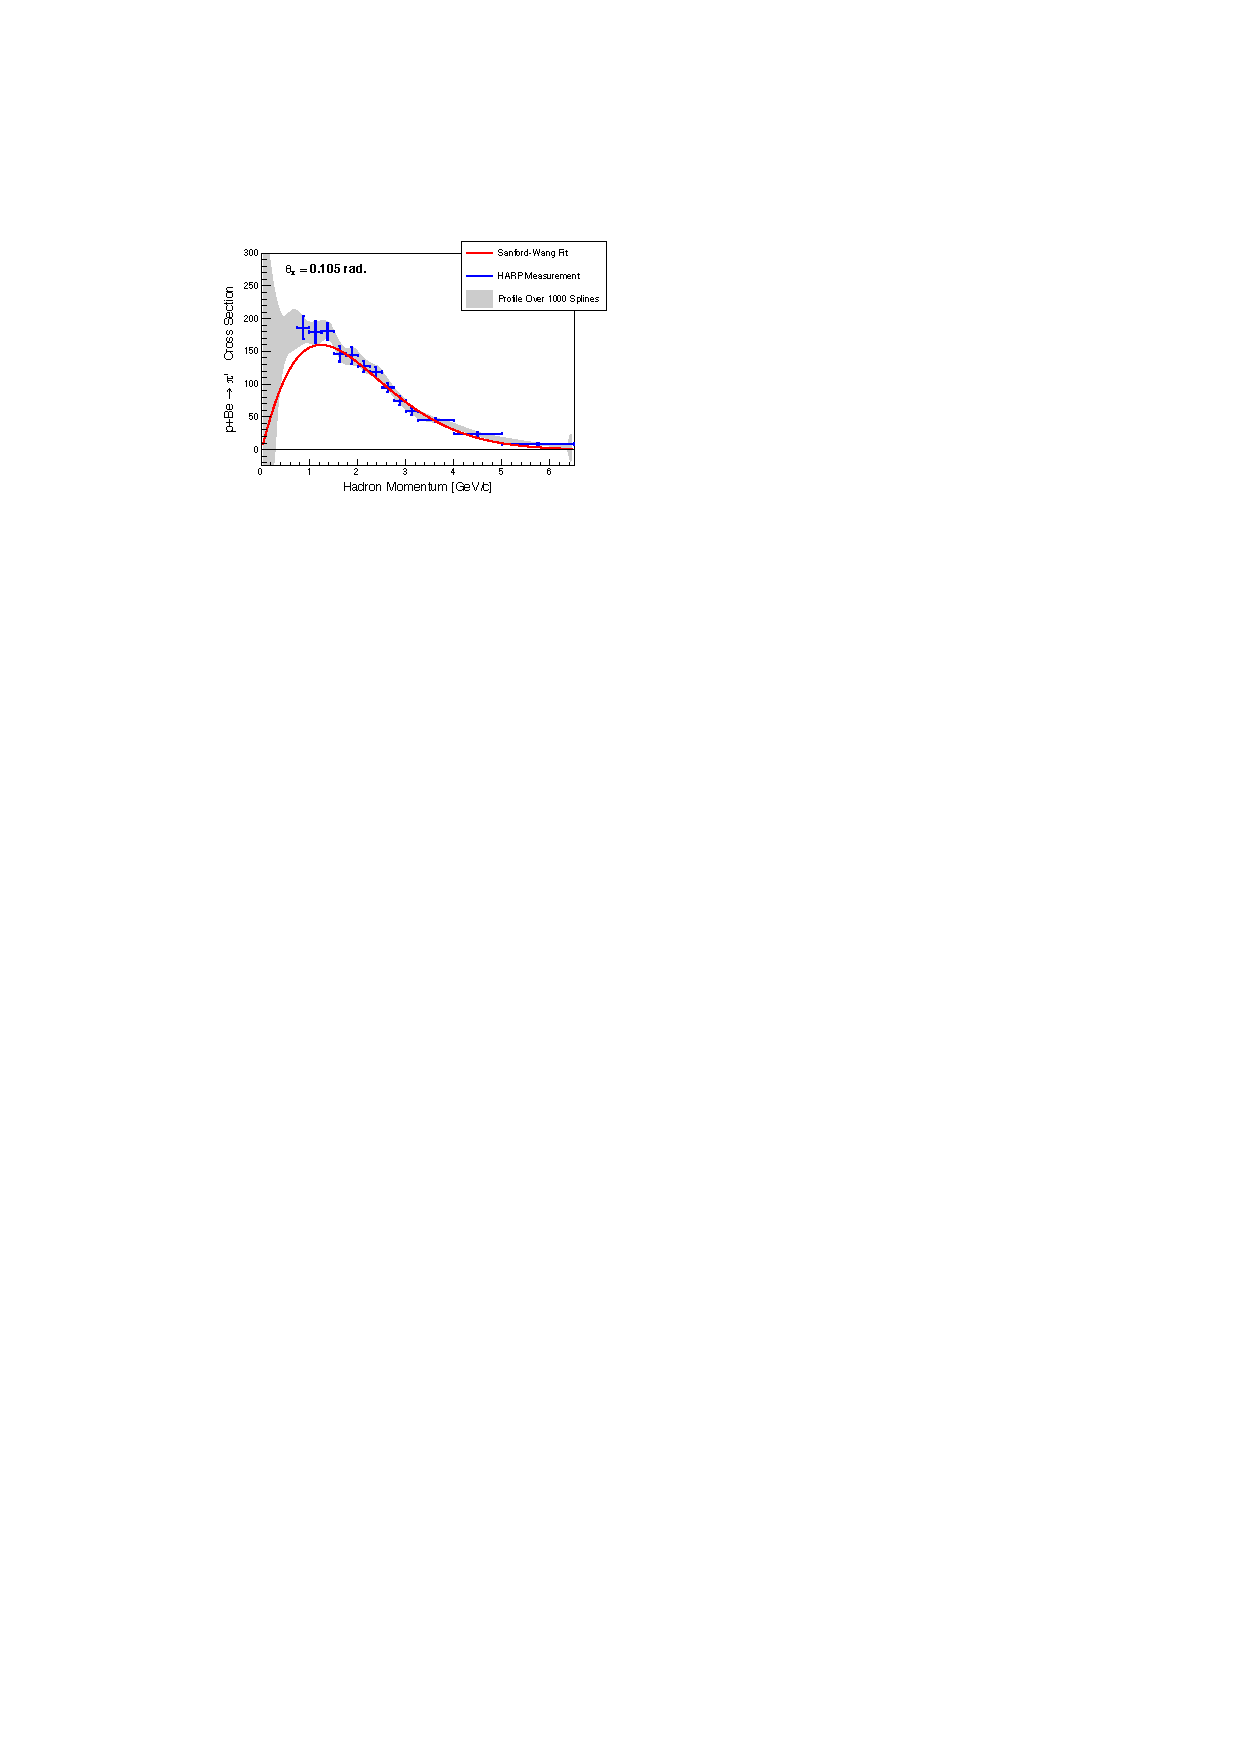
\includegraphics[width=0.75\linewidth]{figures/harp.pdf}
\caption{Pion production at a fixed angle as measured by the HARP experiment and fit with the Sanford-Wang parametrisation.}\label{fig:harp}
\end{figure}

In this case, the nominal value is considered as the central value in the covariance matrix definition of Eq. \ref{eq:covariance}.
The flux-related uncertainty in the number of simulated selected events (no beam-off data) before the background rejection is 12.3\%.

Also in this case the correlation matrix in Figure \ref{fig:corr_flux} shows that the flux systematic effect are positively correlated in the $E_{\mathrm{deposited}}$ bins, which means they generally increase of decrease the total number of neutrino interactions. 

\begin{figure}[htbp]
  \begin{center}
    \begin{subfigure}{0.49\textwidth}
      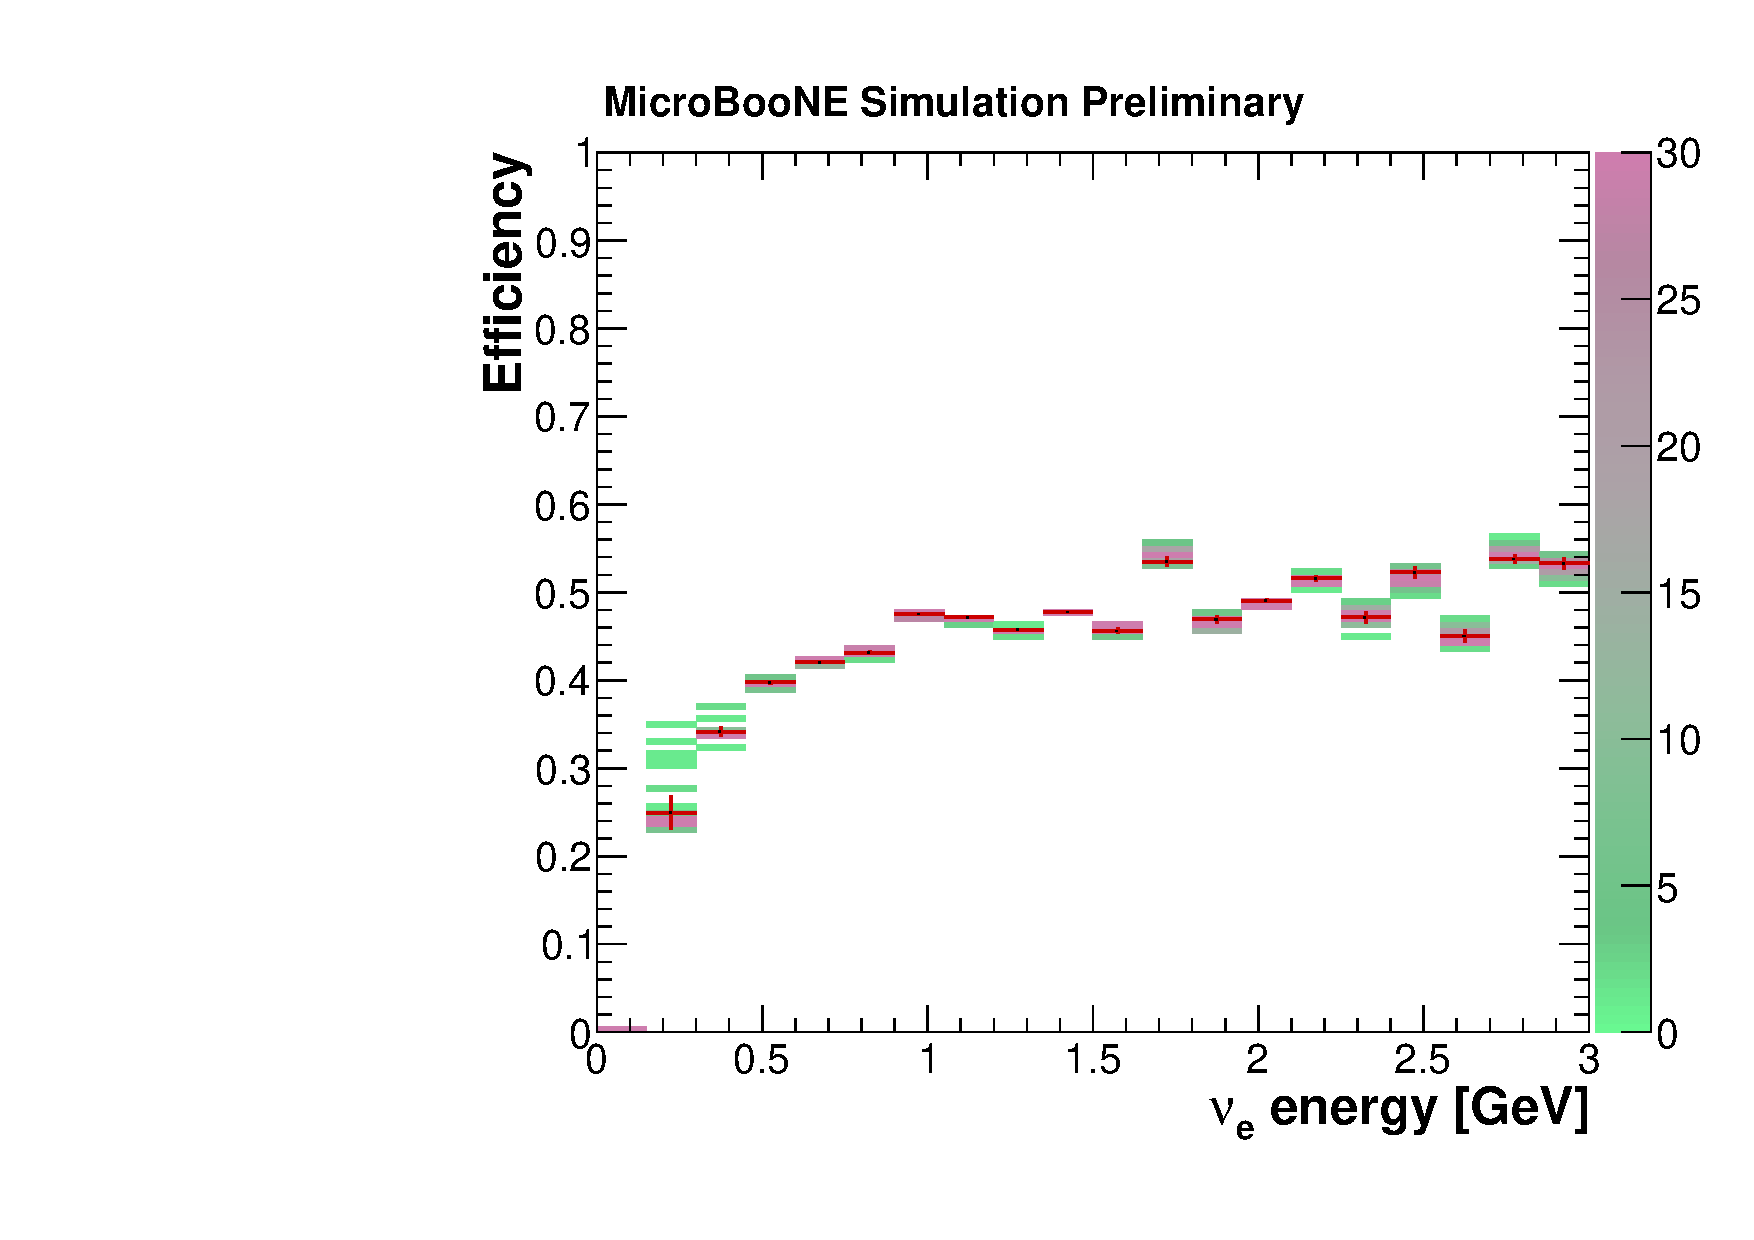
\includegraphics[width=\linewidth]{figures/eff_ene_flux.pdf}
      \caption{$\nu_{e}$ CC0$\pi$-Np selection efficiency.}  \label{fig:eff_flux}
    \end{subfigure}\hfill
    \begin{subfigure}{0.49\textwidth}
      \vspace{0.5em}
      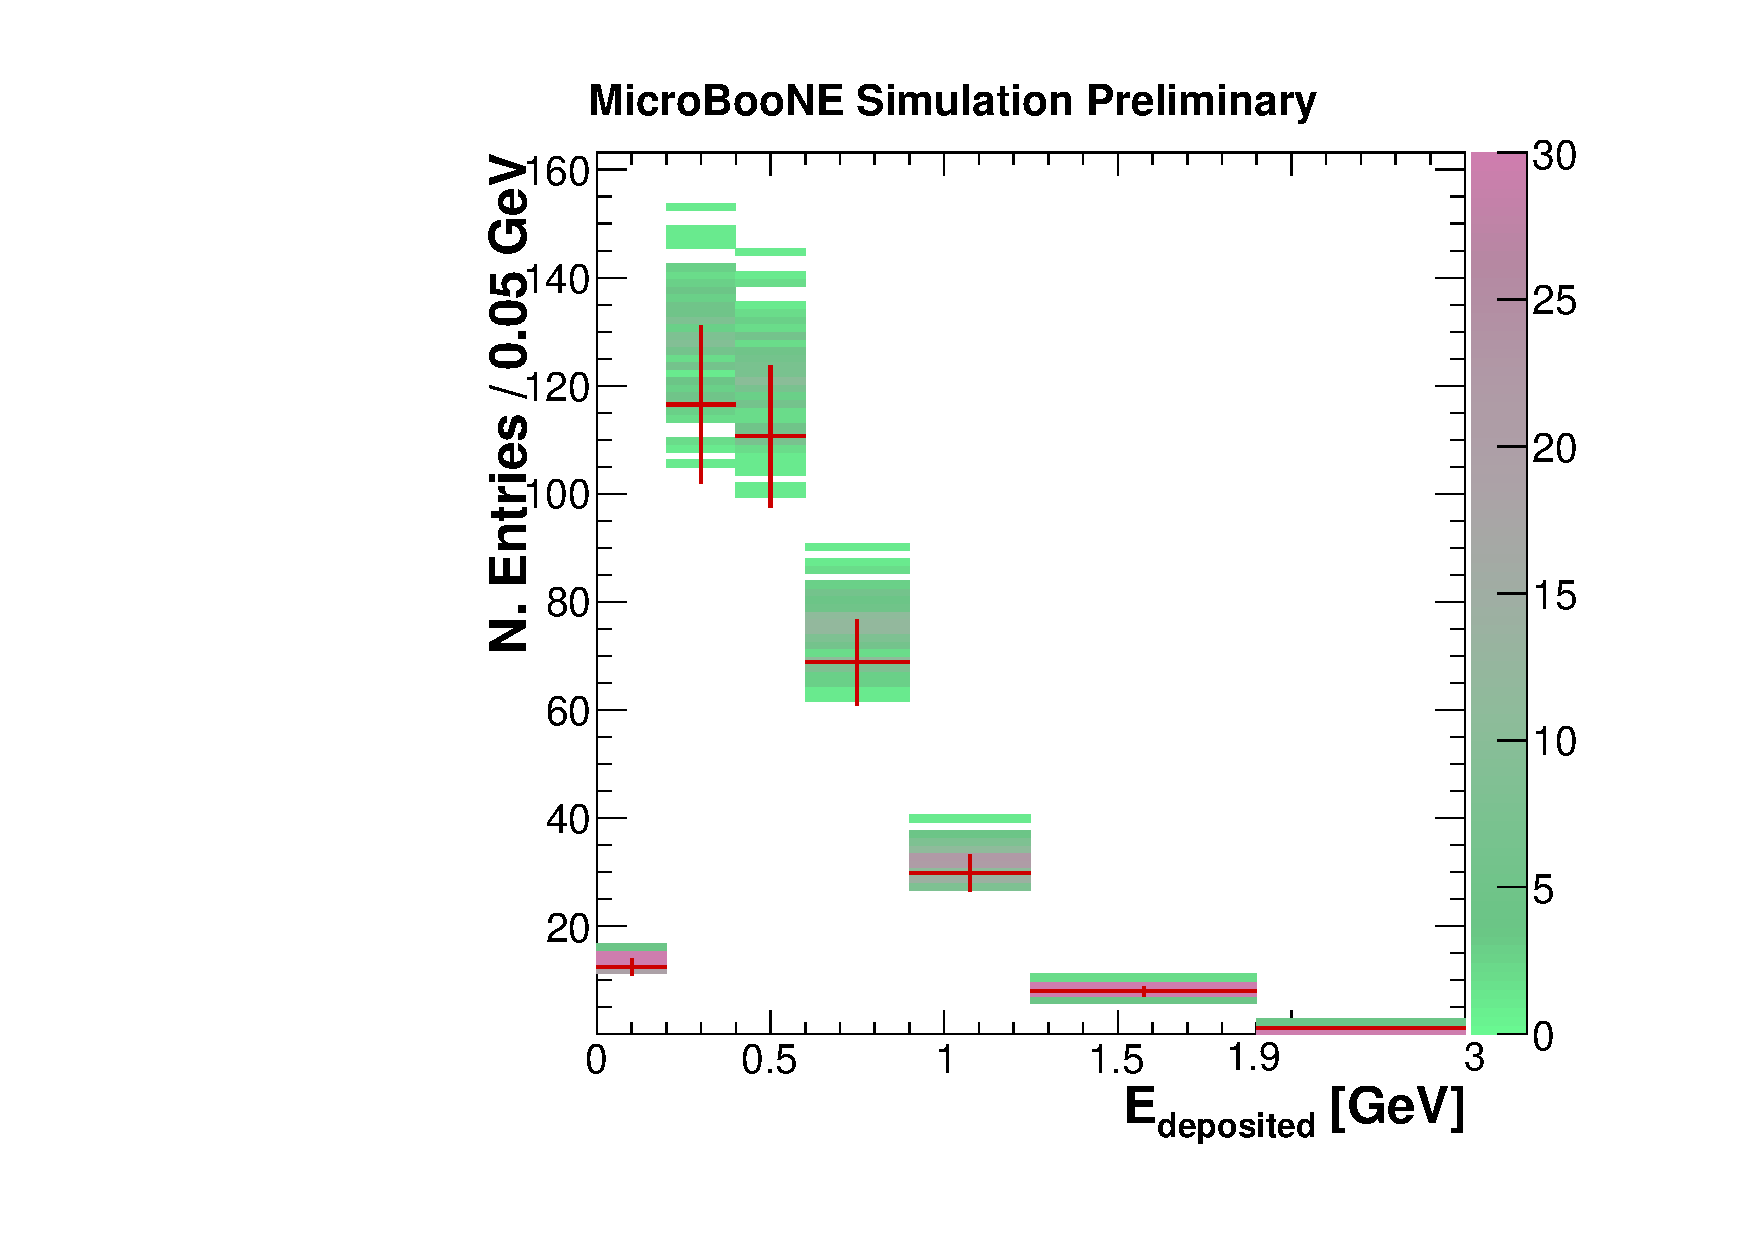
\includegraphics[width=\linewidth]{figures/reco_flux.pdf}
      \caption{Energy spectrum of the selected events.}  \label{fig:reco_flux}
    \end{subfigure}
    \begin{subfigure}{0.49\textwidth}
      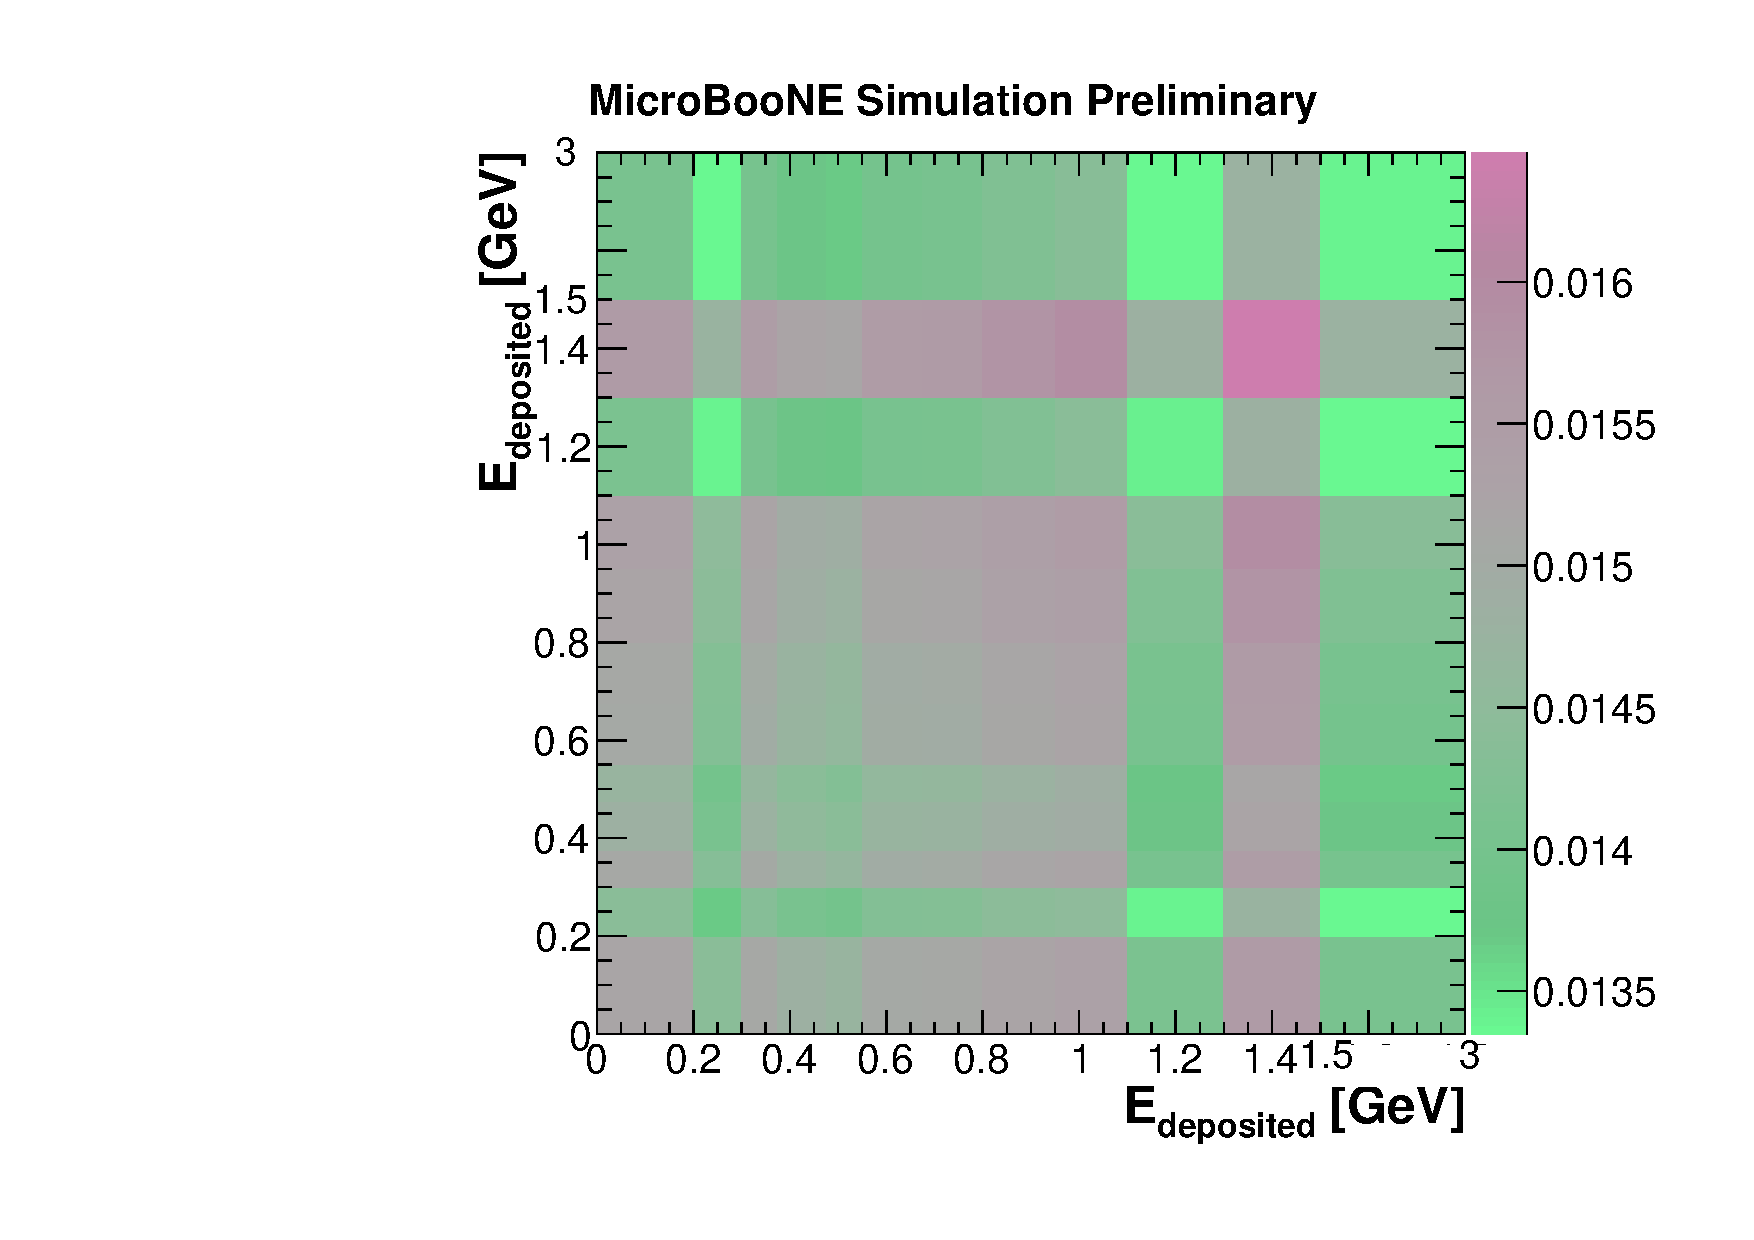
\includegraphics[width=\linewidth]{figures/frac_flux.pdf}
      \caption{Fractional covariance matrix.}  \label{fig:frac_flux}
    \end{subfigure}\hfill
    \begin{subfigure}{0.49\textwidth}
      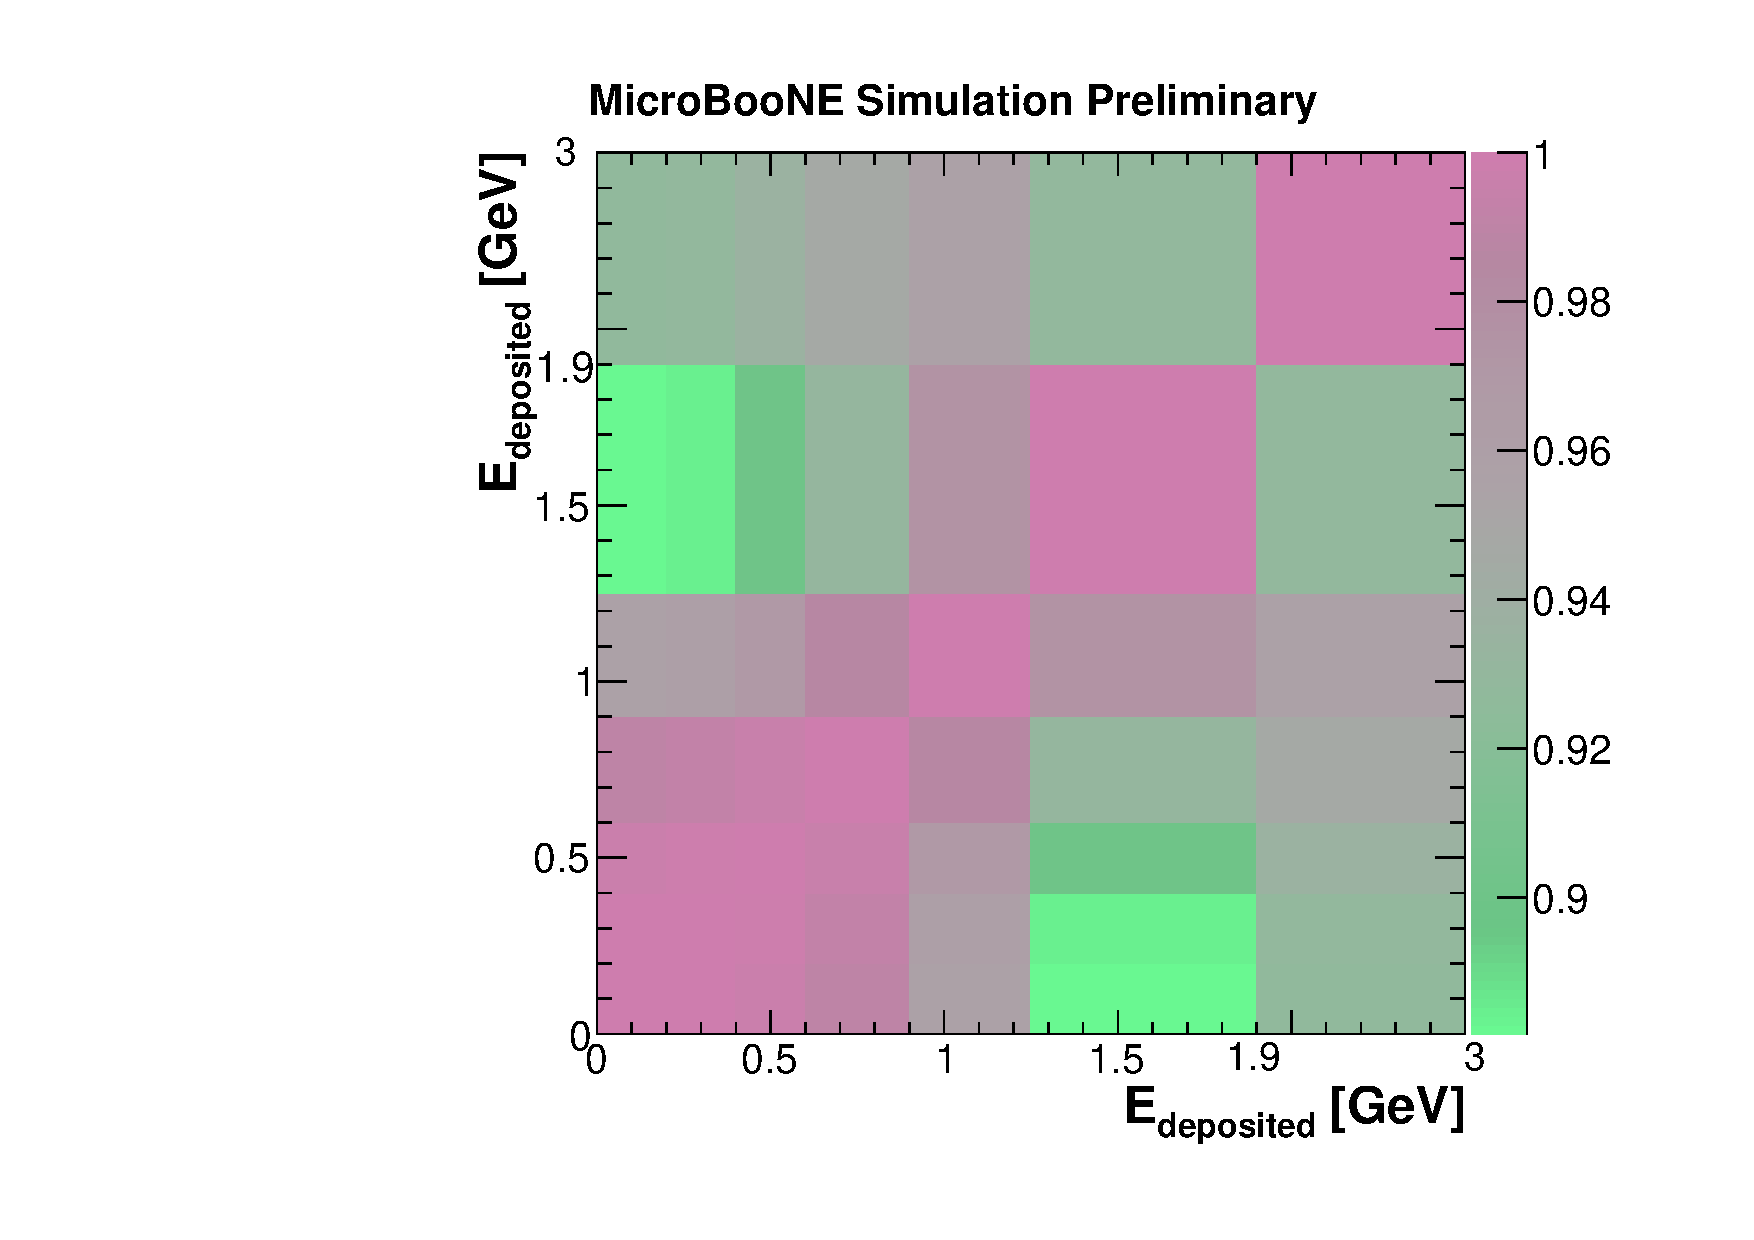
\includegraphics[width=\linewidth]{figures/corr_flux.pdf}
      \caption{Correlation matrix.}  \label{fig:corr_flux}
    \end{subfigure}
    \caption{Selection efficiency, reconstructed energy spectrum, fractional covariance matrix, and correlation matrix obtained by varying the BNB flux parameters in 100 simulated universes. The colour scale for the selection efficiency and the energy spectrum corresponds to the number of universes. The red bars correspond to the central value and its flux systematic uncertainty only. The data beam-off sample is not included in these plots.}\label{fig:flux_sys}
	\end{center}
\end{figure}


\section{Cross-section systematic uncertainties}
In order to estimate the cross-section systematic uncertainties, the standard GENIE parameters described in the Chapter 9 of the GENIE User Manual \cite{Andreopoulos:2015wxa} are simultaneously varied within their uncertainties in $N_{u} = 100$ simulated universes. The correlation between the parameters is accounted for internally by GENIE. A calculated \emph{weight} gets assigned to each universe, which is applied when filling the histograms of the reconstructed quantities. The uncertainties shown here do not include systematic effects associated with Random Phase Approximation (RPA) and with Meson Exchange Current (MEC) interactions. RPA refers to long-range multi-nucleon correlations which suppress the neutrino-nucleon cross-section at low-exchanged momentum $Q^2$ \cite{Nieves:2011pp}. MEC interactions involve the scatter between the neutrino and a correlated pair of nucleons (\emph{2p-2h}) \cite{Bodek:2011ps}. These two systematic effects will be quantified in a future version of the analysis.

Figure \ref{fig:eff_genie} shows the central value of the $\nu_{e}$ CC0$\pi$-Np selection efficiency and the corresponding value for each GENIE variation universe. The variation in this case is expected to be small, since we are essentially dividing two distributions (passed and total) with similar weights. Figure \ref{fig:reco_genie} and Figure \ref{fig:frac_genie} show that the variations in the reconstructed energy spectrum are larger at lower energies, which is the energy region most affected by the GENIE parameters uncertainties. The GENIE-related uncertainty in the number of simulated selected events (no beam-off data) before the background rejection is 7.9\%.
The correlation matrix in Figure \ref{fig:corr_genie} shows that the bins are mostly positively correlated. This means that the variations of the GENIE parameters has in our case mostly a normalisation effect (i.e. they change the total number of events). 

\begin{figure}[htbp]
  \begin{center}
    \begin{subfigure}{0.49\textwidth}
      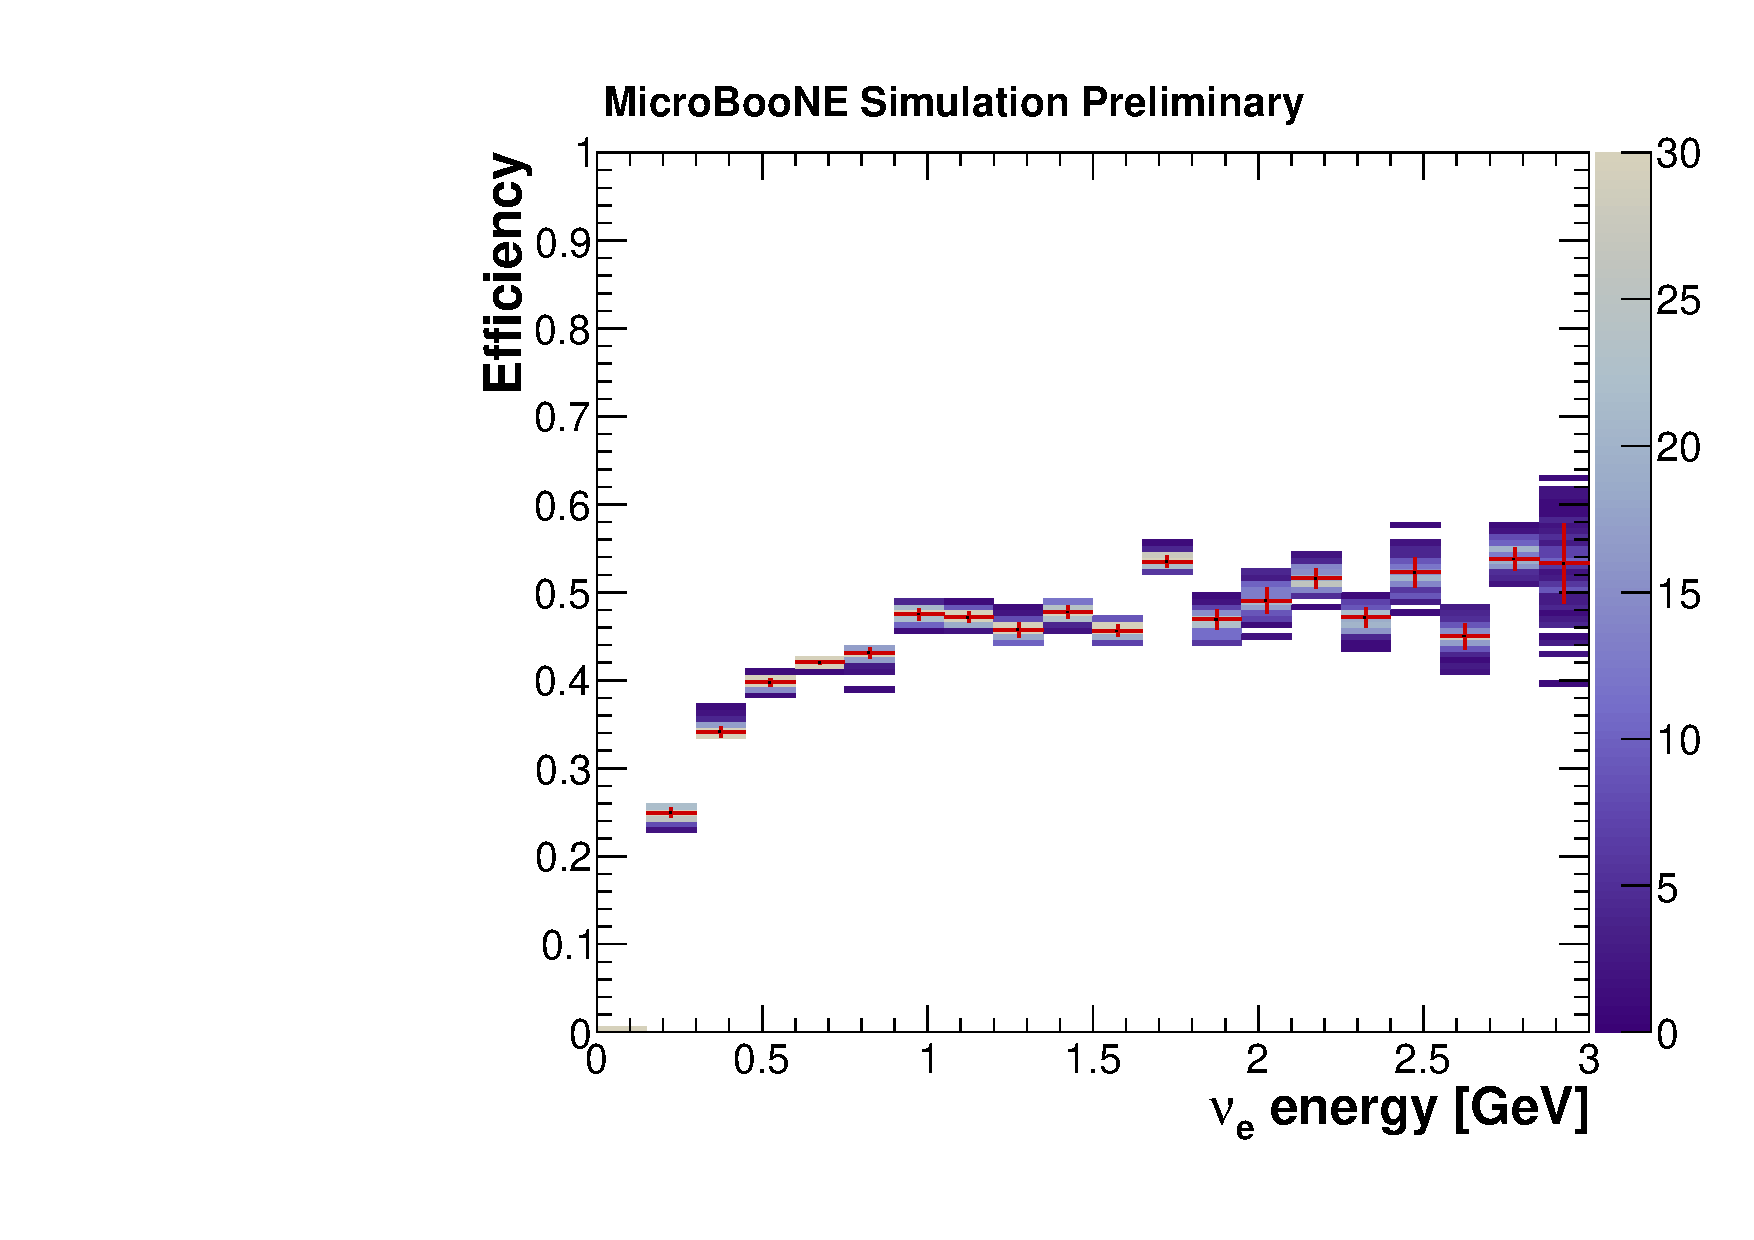
\includegraphics[width=\linewidth]{figures/eff_ene_genie.pdf}
      \caption{$\nu_{e}$ CC0$\pi$-Np selection efficiency.}  \label{fig:eff_genie}
    \end{subfigure}\hfill
    \begin{subfigure}{0.49\textwidth}
      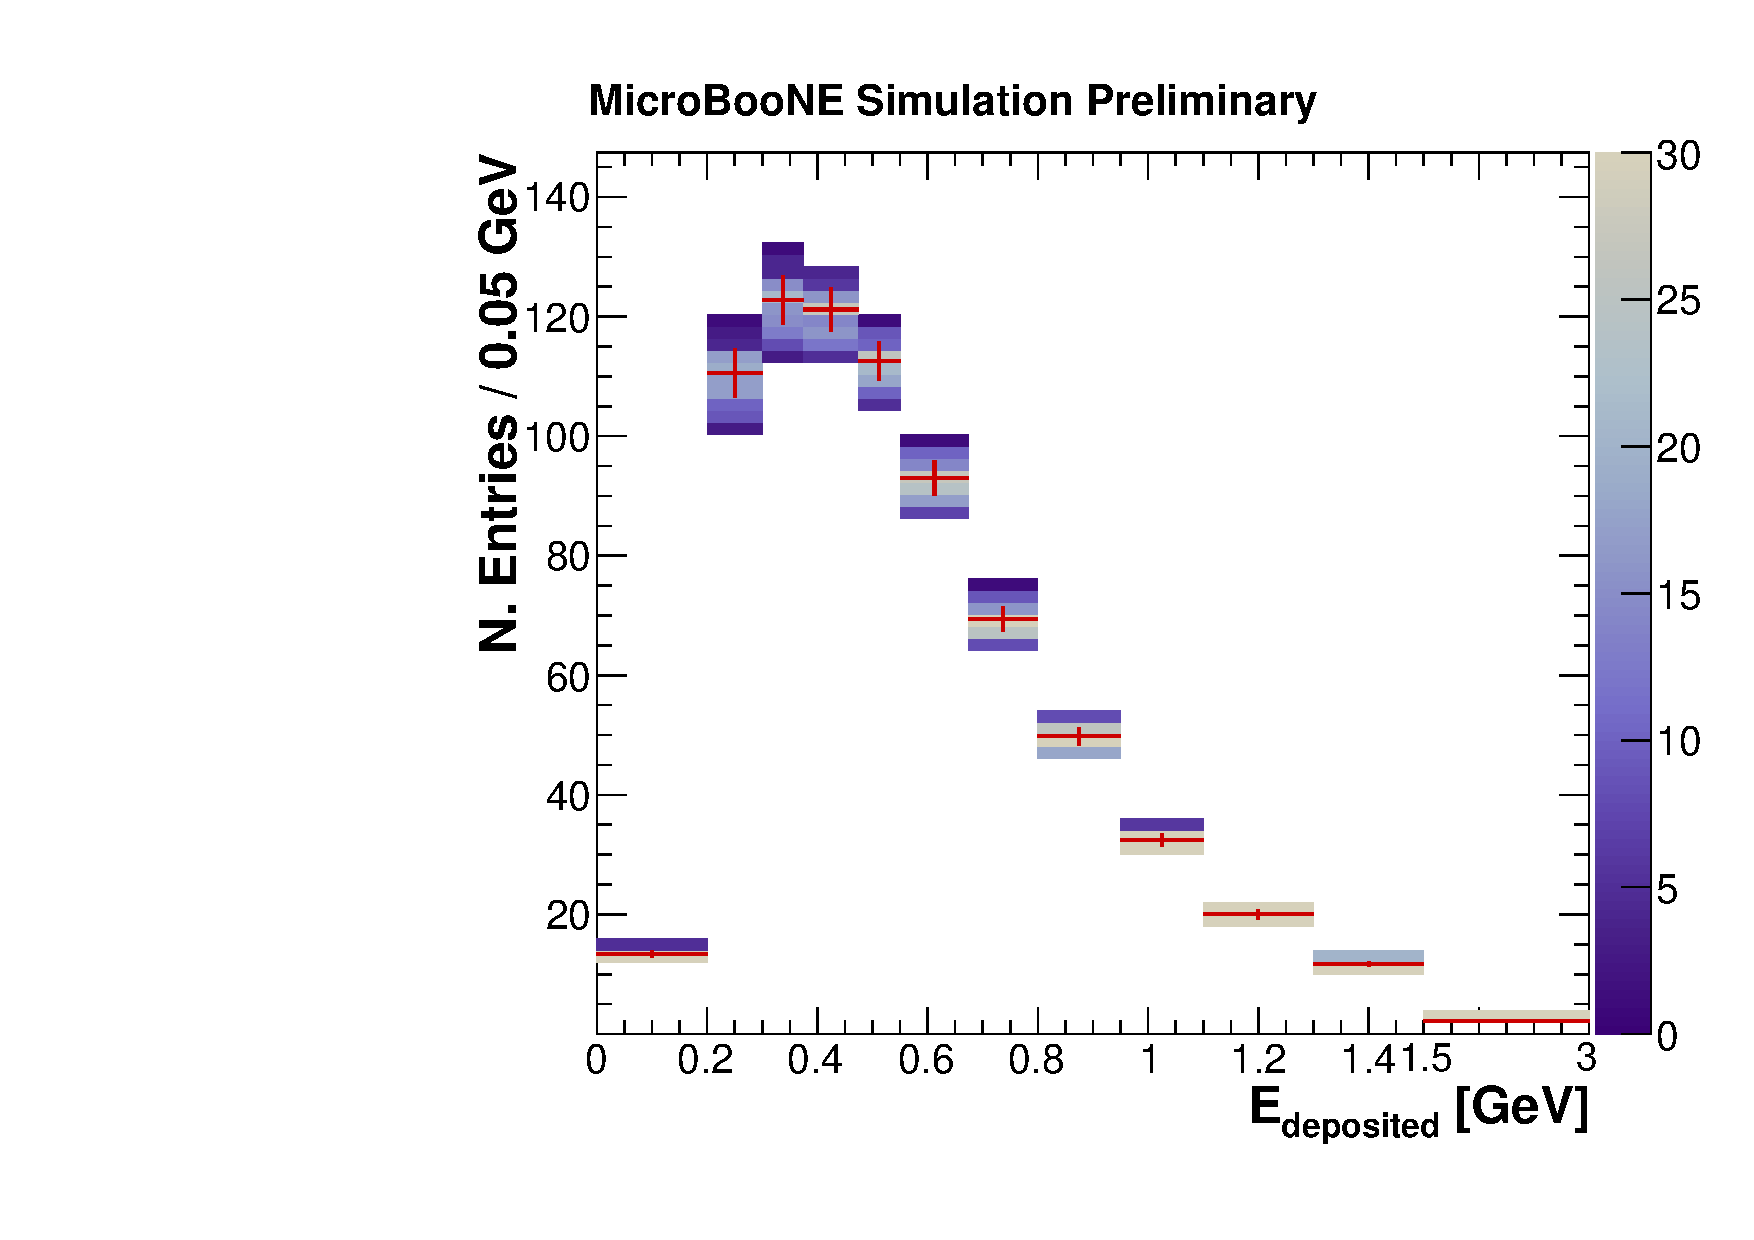
\includegraphics[width=\linewidth]{figures/reco_genie.pdf}
      \caption{Energy spectrum of the selected events.}  \label{fig:reco_genie}
    \end{subfigure}
    \begin{subfigure}{0.49\textwidth}
      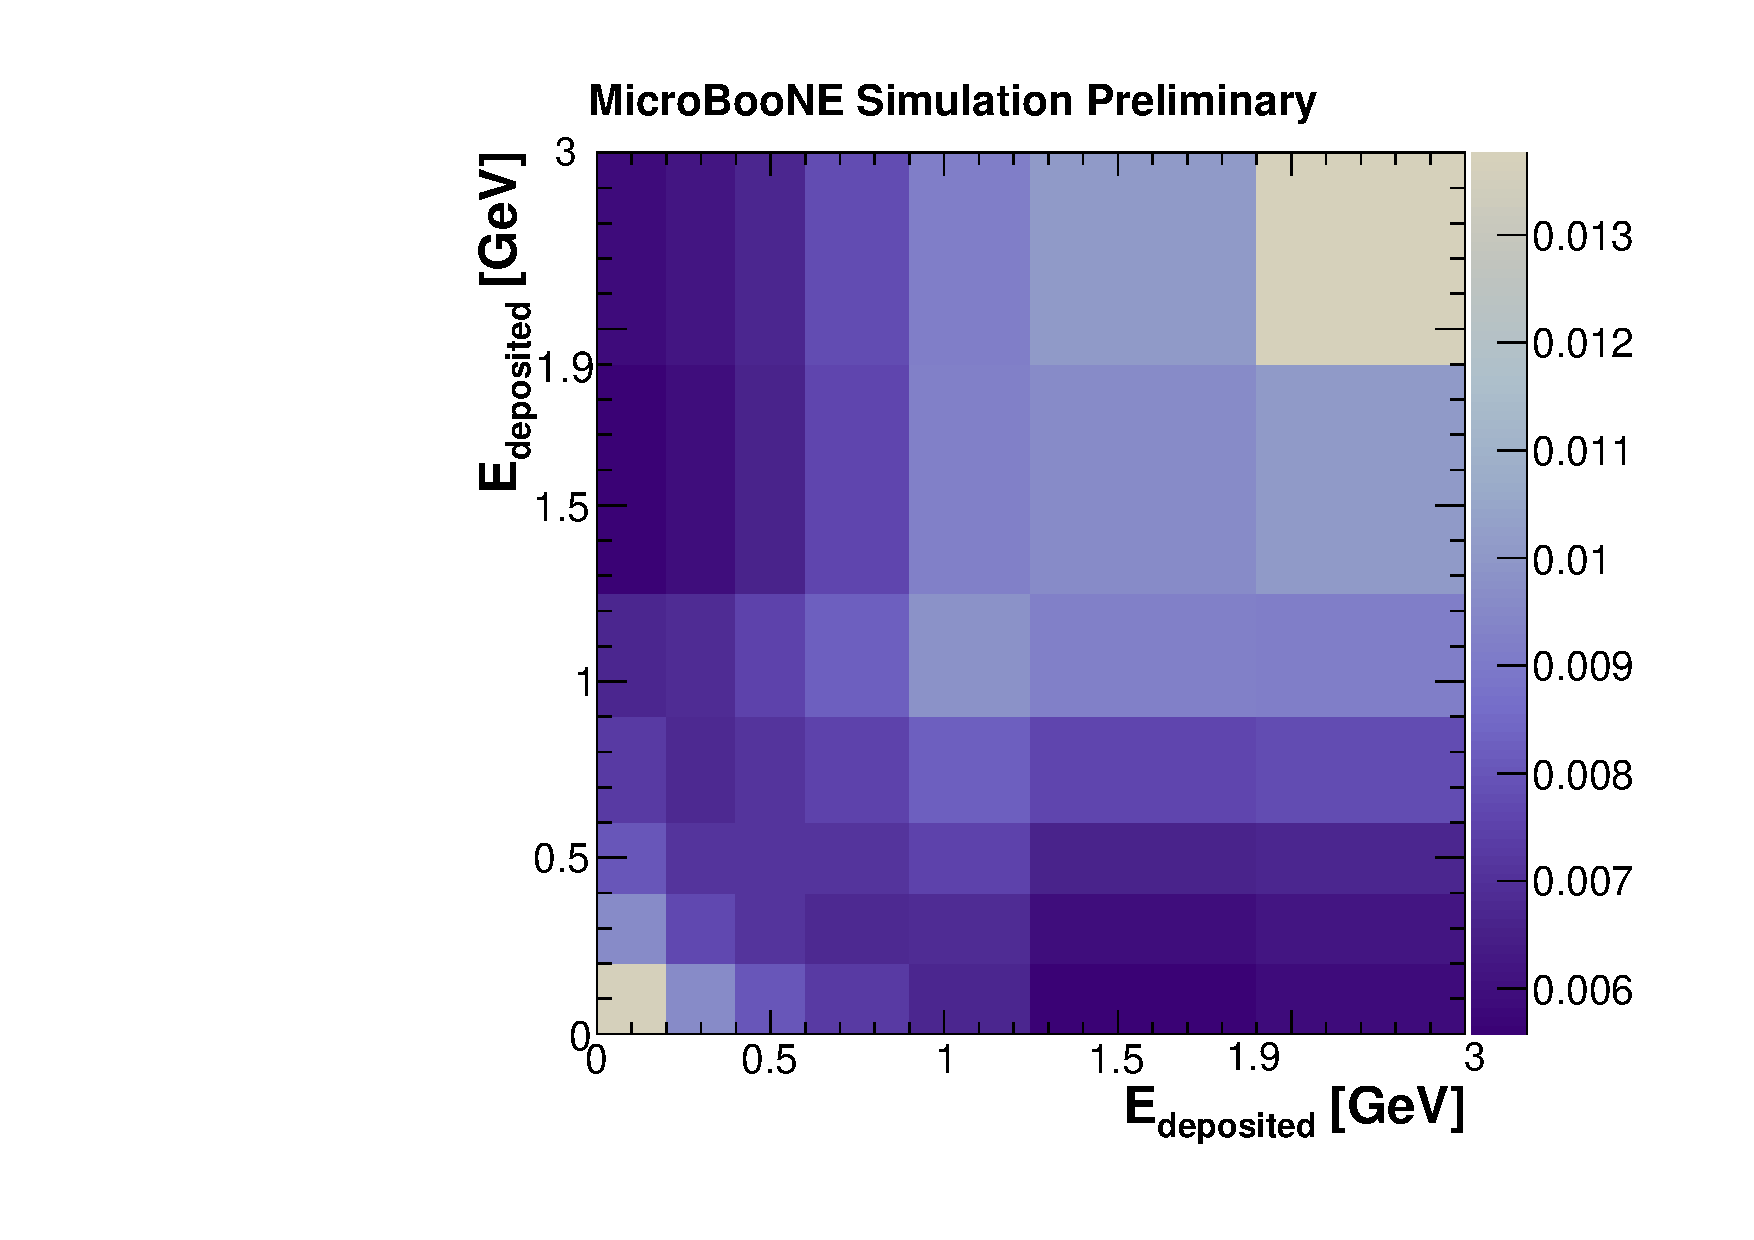
\includegraphics[width=\linewidth]{figures/frac_genie.pdf}
      \caption{Fractional covariance matrix.}\label{fig:frac_genie}
    \end{subfigure}\hfill
    \begin{subfigure}{0.49\textwidth}
      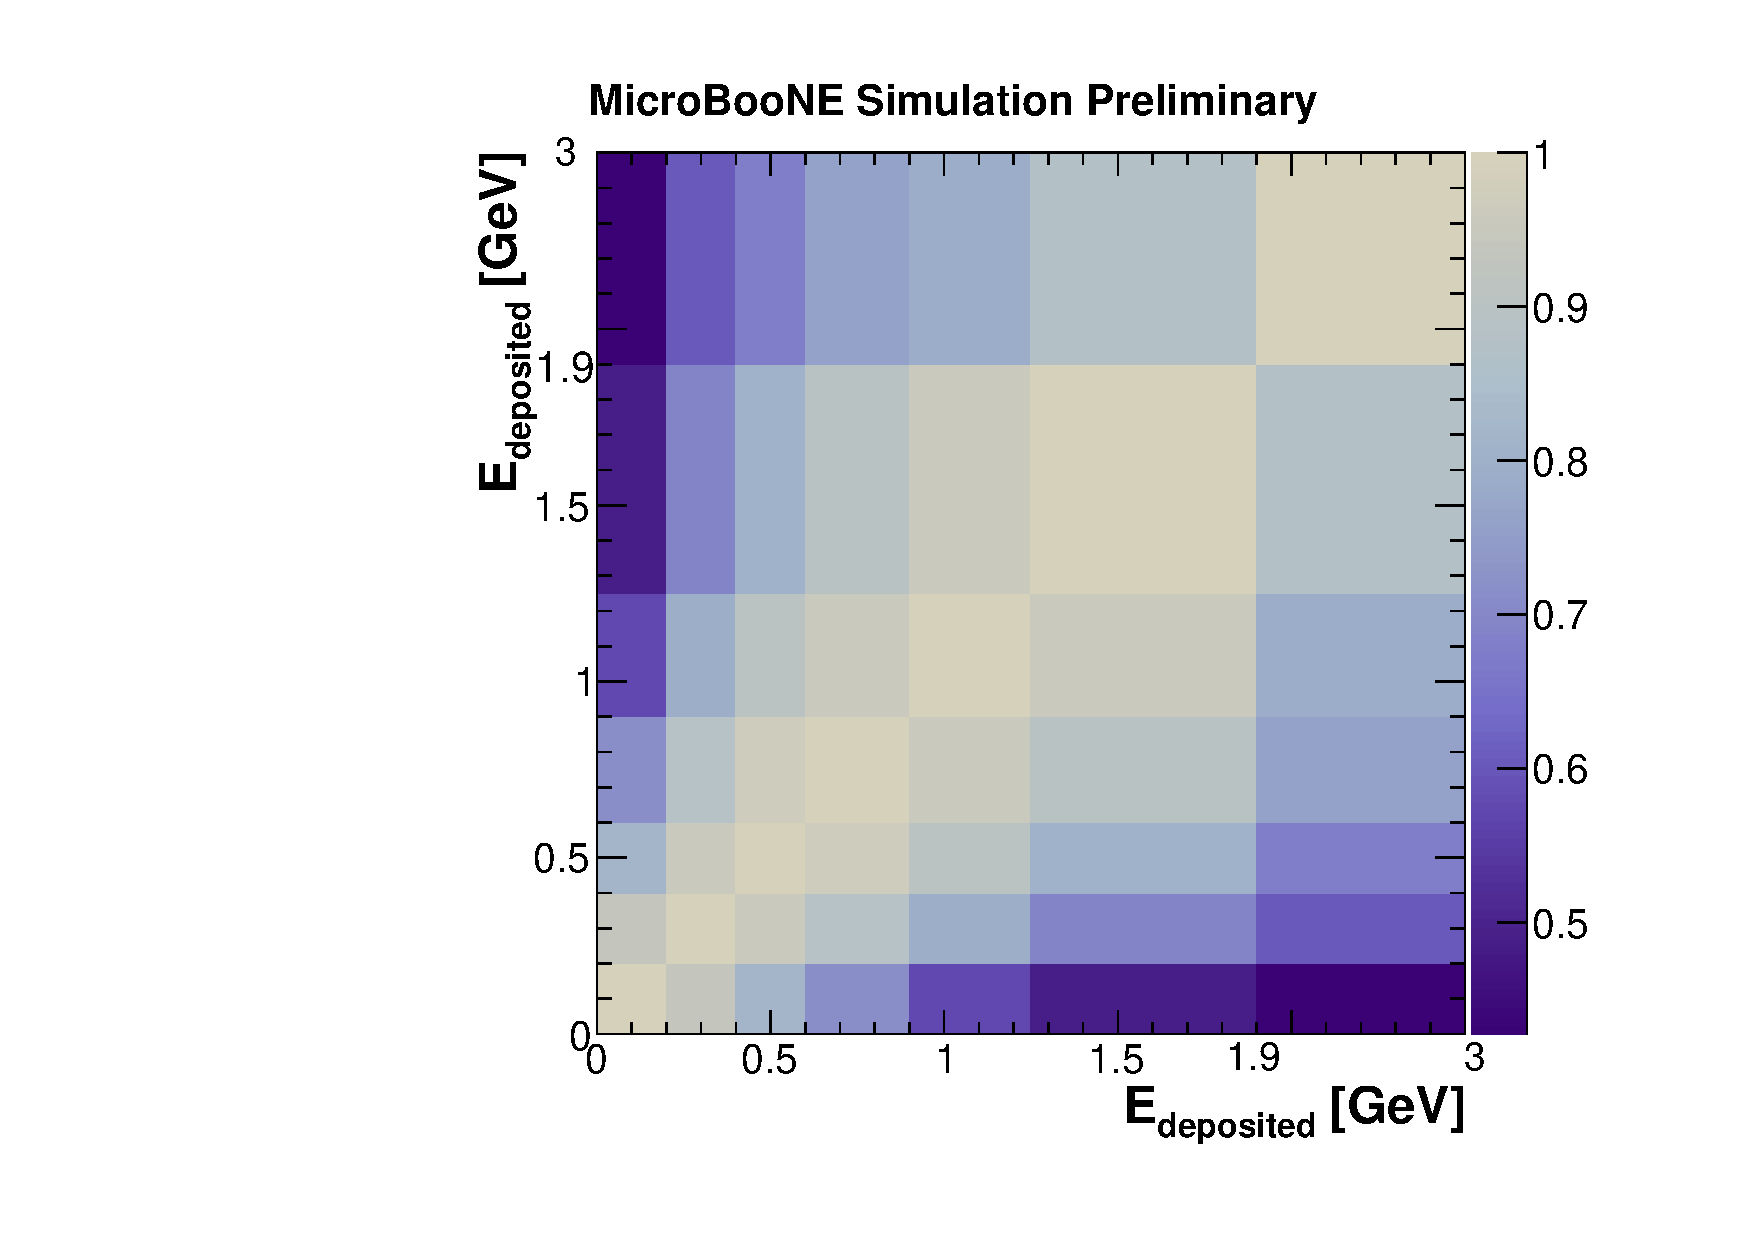
\includegraphics[width=\linewidth]{figures/corr_genie.pdf}
      \caption{Correlation matrix.}\label{fig:corr_genie}
    \end{subfigure}
    \caption{Selection efficiency, reconstructed energy spectrum, fractional covariance matrix, and correlation matrix obtained by varying the standard GENIE parameters in 100 simulated universes. The colour scale for the selection efficiency and the energy spectrum corresponds to the number of universes. The red bars correspond to the central value and its cross-section systematic uncertainty only. Events with MEC interactions are not included in these plots and the uncertainties do not include RPA effects. The data beam-off sample is not included in these plots.} \label{fig:genie_sys}
	\end{center}
\end{figure}

\section{Detector systematic uncertainties}\label{sec:detector_sys}
The detector systematic uncertainties have been measured by simulating several samples where a single detector parameter is varied by its estimated $\pm1\sigma$ uncertainty or where a different physics model is used. The detector variations taken into consideration are:
\begin{description}
\item[Space-charge effect.] The $x$-dependence of the space-charge effect is estimated with a data-driven procedure and its magnitude is scaled by 0.7.
\item[Dynamic Induced Charge.] Improved simulation of the induction of charge on the neighbouring wires.
\item[Light simulation.] Improved simulation of the light production in the detector.
\item[Saturated channels.] Channels that tend to saturate are turned off in the simulation.
\item[Misconfigured channels.] Channels with misconfigured ASIC gains and shaping are turned off in the simulation.
\item[Electron lifetime.] Lifetime of the electron in the detector is reduced to 10~ms, which corresponds to a lower LAr purity.
\item[Recombination model.] The Birks model of recombination \cite{Amoruso:2004dy} is used instead of the modified box model \cite{Acciarri:2013met}. 
\item[Longitudinal diffusion.] The longitude diffusion is varied by $\pm1\sigma$ of its estimated uncertainty.
\item[Transverse diffusion.] The transverse diffusion is varied by $\pm1\sigma$ of its estimated uncertainty.
\item[Wire noise.] The amount of noise on the wires is varied by $\pm1\sigma$ of its estimated uncertainty.
\item[PE noise.] The amount of single-PE noise in the PMTs is varied by $\pm1\sigma$ of its estimated uncertainty.
\item[Cryostat light.] The light outside the TPC but inside the cryostat is increased by 20\%.
\item[Wire response.] The wire response functions are squeezed by 20\%.
\end{description}

In this case, the covariance matrix is calculated using the definition in Eq. \ref{eq:cov_det}. The fractional covariance matrix and the reconstructed energy spectrum are shown in Figure \ref{fig:frac_det} and Figure \ref{fig:reco_det}, respectively.
The uncertainty related to the detector systematic effects in the number of simulated selected events is 24.0\%. The limited size of the detector variation samples does not allow us to calculate the covariance matrix after the rectangular or BDTs cuts. For this reason, a flat 24.0\% detector uncertainty is applied to the simulated events not rejected by the rectangular of BDTs cuts. This high detector systematic uncertainties reflect our knowledge of the detector when the samples were generated (August 2018). However, we are now able to simulate the detector more precisely, by including e.g. a full data-driven map of the space-charge effect and the charge induction on neighbouring wires, which will lead us to significantly smaller systematic uncertainties. %Detector variation samples with a higher statistics of $\nu_e$ interactions are not currently available and the detector uncertainty for the $\nu_e$~CC0$\pi$-Np and $\nu_e$~CC categories is assumed to be 24.0\%.

The details of the detector systematic uncertainties are listed in Table \ref{tab:det_bkg}. In this case, the detector variations $\sigma_{\mathrm{det}}$ are defined as:
\begin{equation}
    \sigma_{\mathrm{det}} = \frac{x^{cv} - x^s}{x^{cv}},
\end{equation}
where $x^{cv}$ is the number of the selected events in the central value sample and $x^s$ is the number of selected events in the variation sample $s$. For the samples where one detector parameter was varied by its $\pm1\sigma$ uncertainty, the larger variation is quoted.

The components showing the largest variations are the \emph{Cosmic}, \emph{Cosmic contaminated}, and \emph{Outside fid. vol.} background categories. In particular, the sample with a different simulation of the space-charge effect causes a variation of the \emph{Cosmic}, \emph{Cosmic contaminated}, and \emph{Outside fid. vol.} components of 28.0\%, 42.0\%, and 32.5\%, respectively. This is expected, since these events are mostly located near the borders of the TPC, so if the magnitude of the space-charge effect is decreased, more events will be shifted towards the borders and then removed by the fiducial volume cut.

The sample with an improved simulation of the charge induced on the neighbouring wires introduces a large variation in the \emph{Beam intrinsic $\nu_{\mu}$} component (19.0\% more events in the detector variation sample). This is because this simulation makes ionisation tracks look more like shower objects, increasing the number of events which satisfy our topology requirement.

The correlation matrix in Figure \ref{fig:corr_det} shows a positive correlation among the $E_{\mathrm{deposited}}$ bins, mainly dominated by the space-charge effect. As explained above, an increase (decrease) in the magnitude of this effect cause an increase (decrease) in the number of cosmogenic background events selected. 

\begin{figure}[htbp]
  \begin{center}
    \begin{subfigure}{0.49\textwidth}
      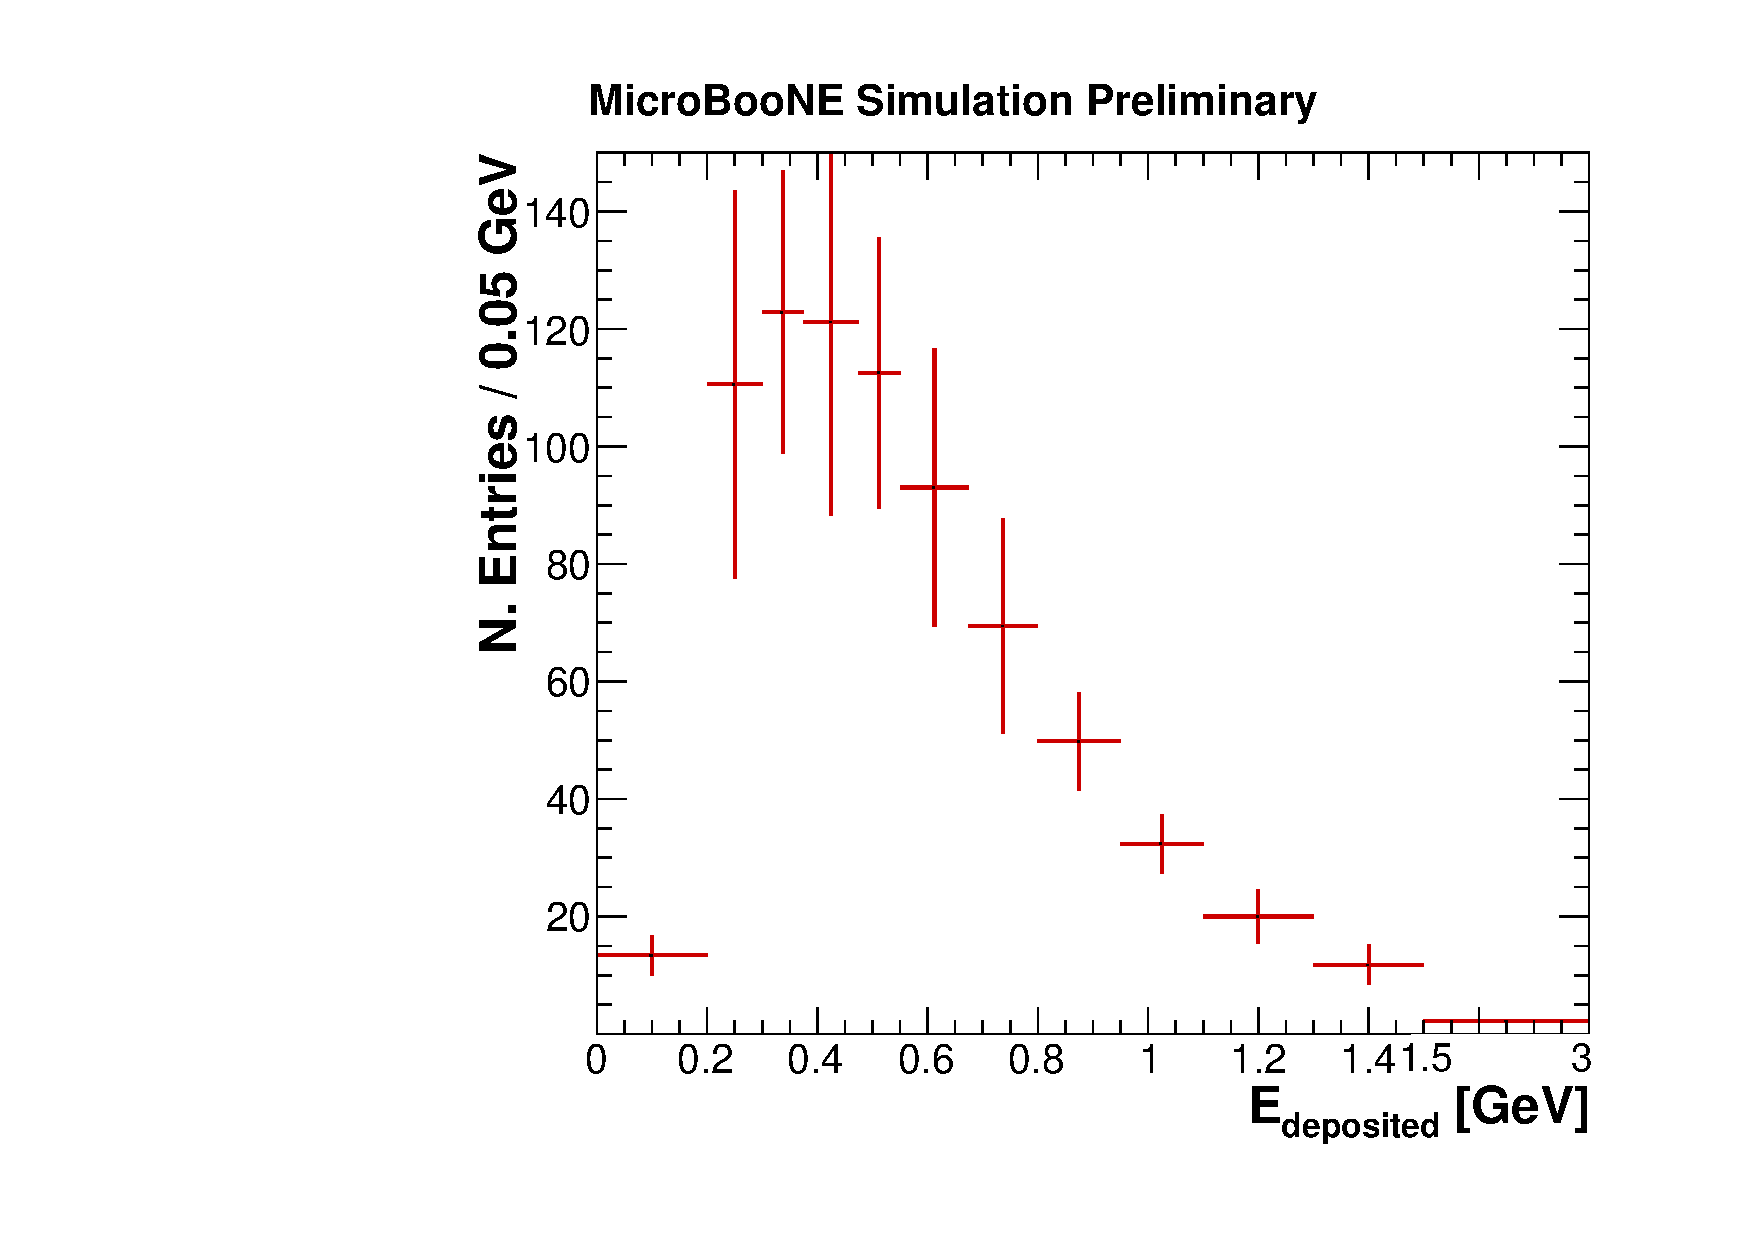
\includegraphics[width=\linewidth]{figures/reco_det.pdf}
      \caption{Energy spectrum of selected events.}  \label{fig:reco_det}
    \end{subfigure}\hfill
    \begin{subfigure}{0.49\textwidth}
      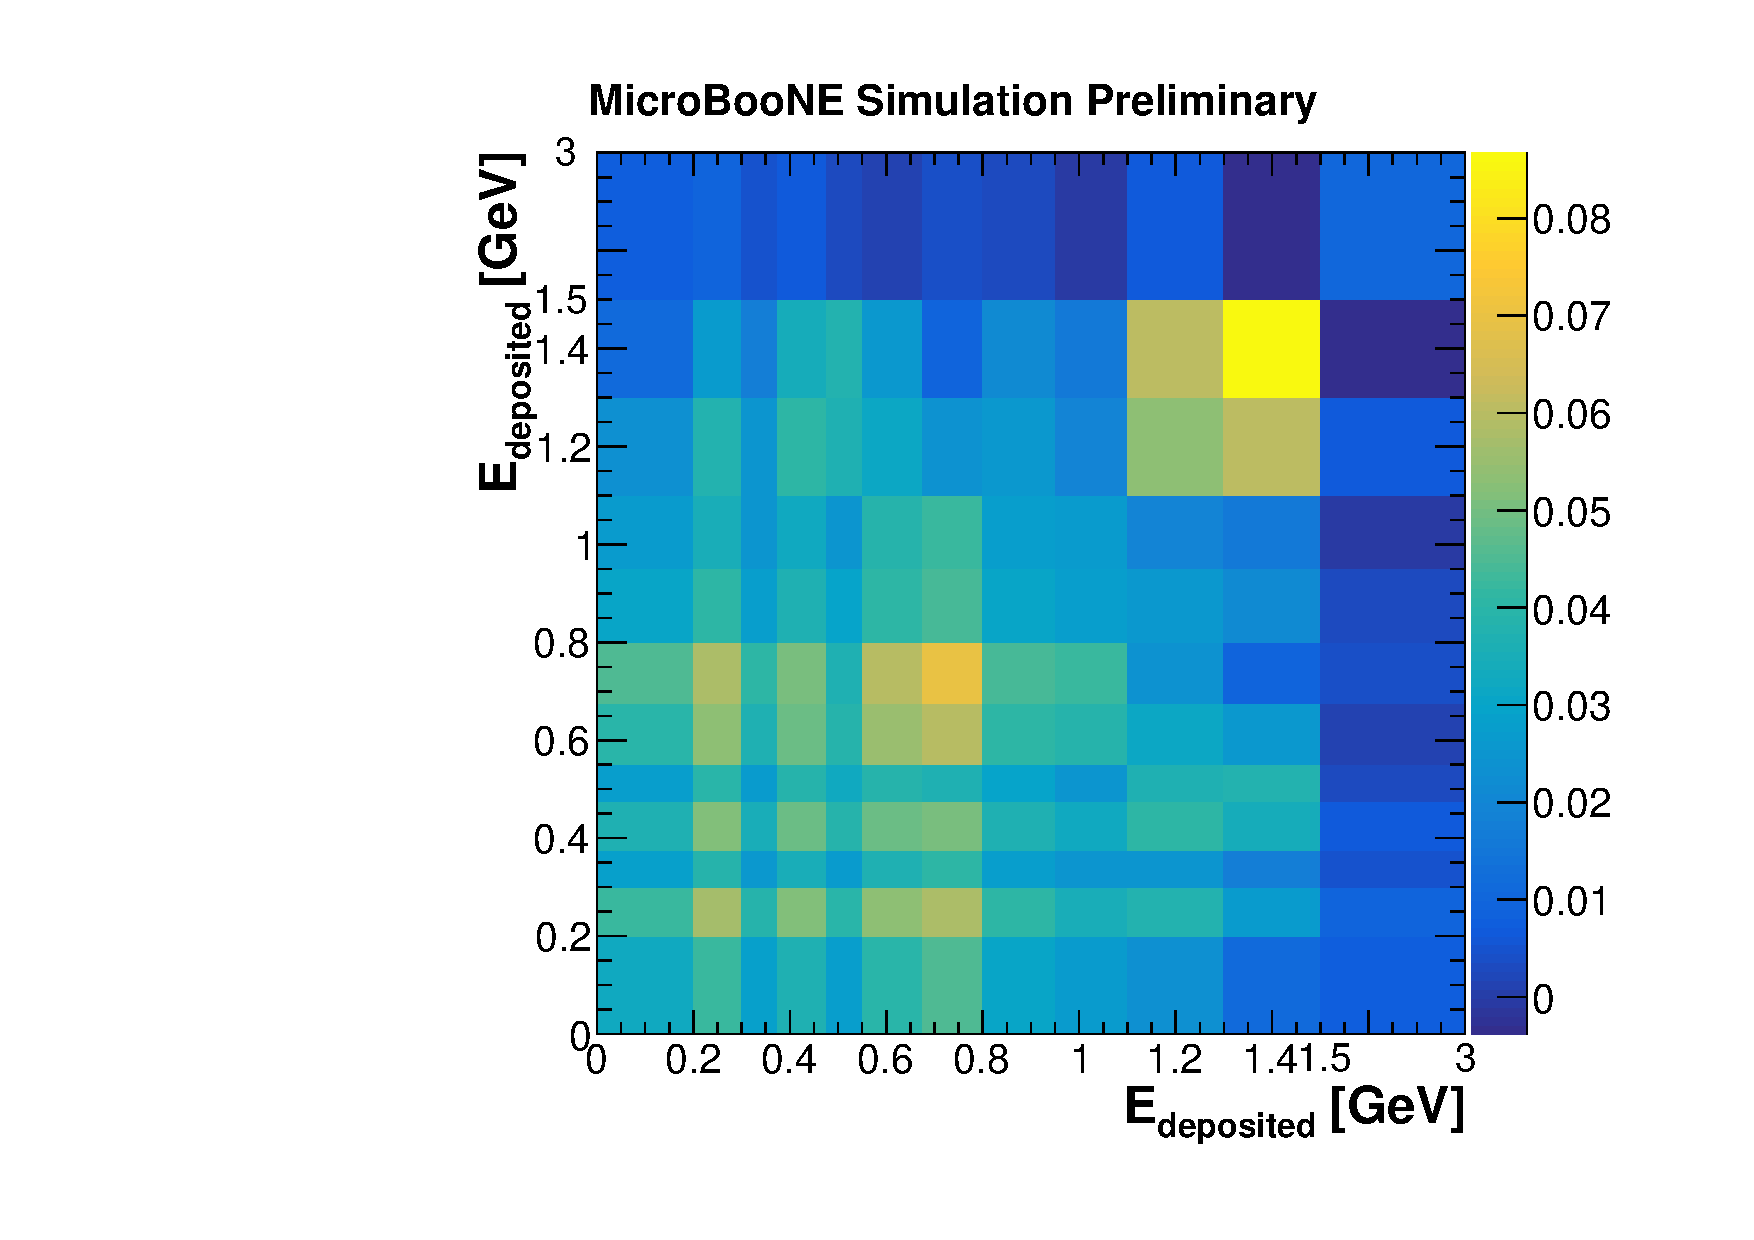
\includegraphics[width=\linewidth]{figures/frac_det.pdf}
      \caption{Fractional covariance matrix.}  \label{fig:frac_det}
    \end{subfigure}
    \begin{subfigure}{0.49\textwidth}
      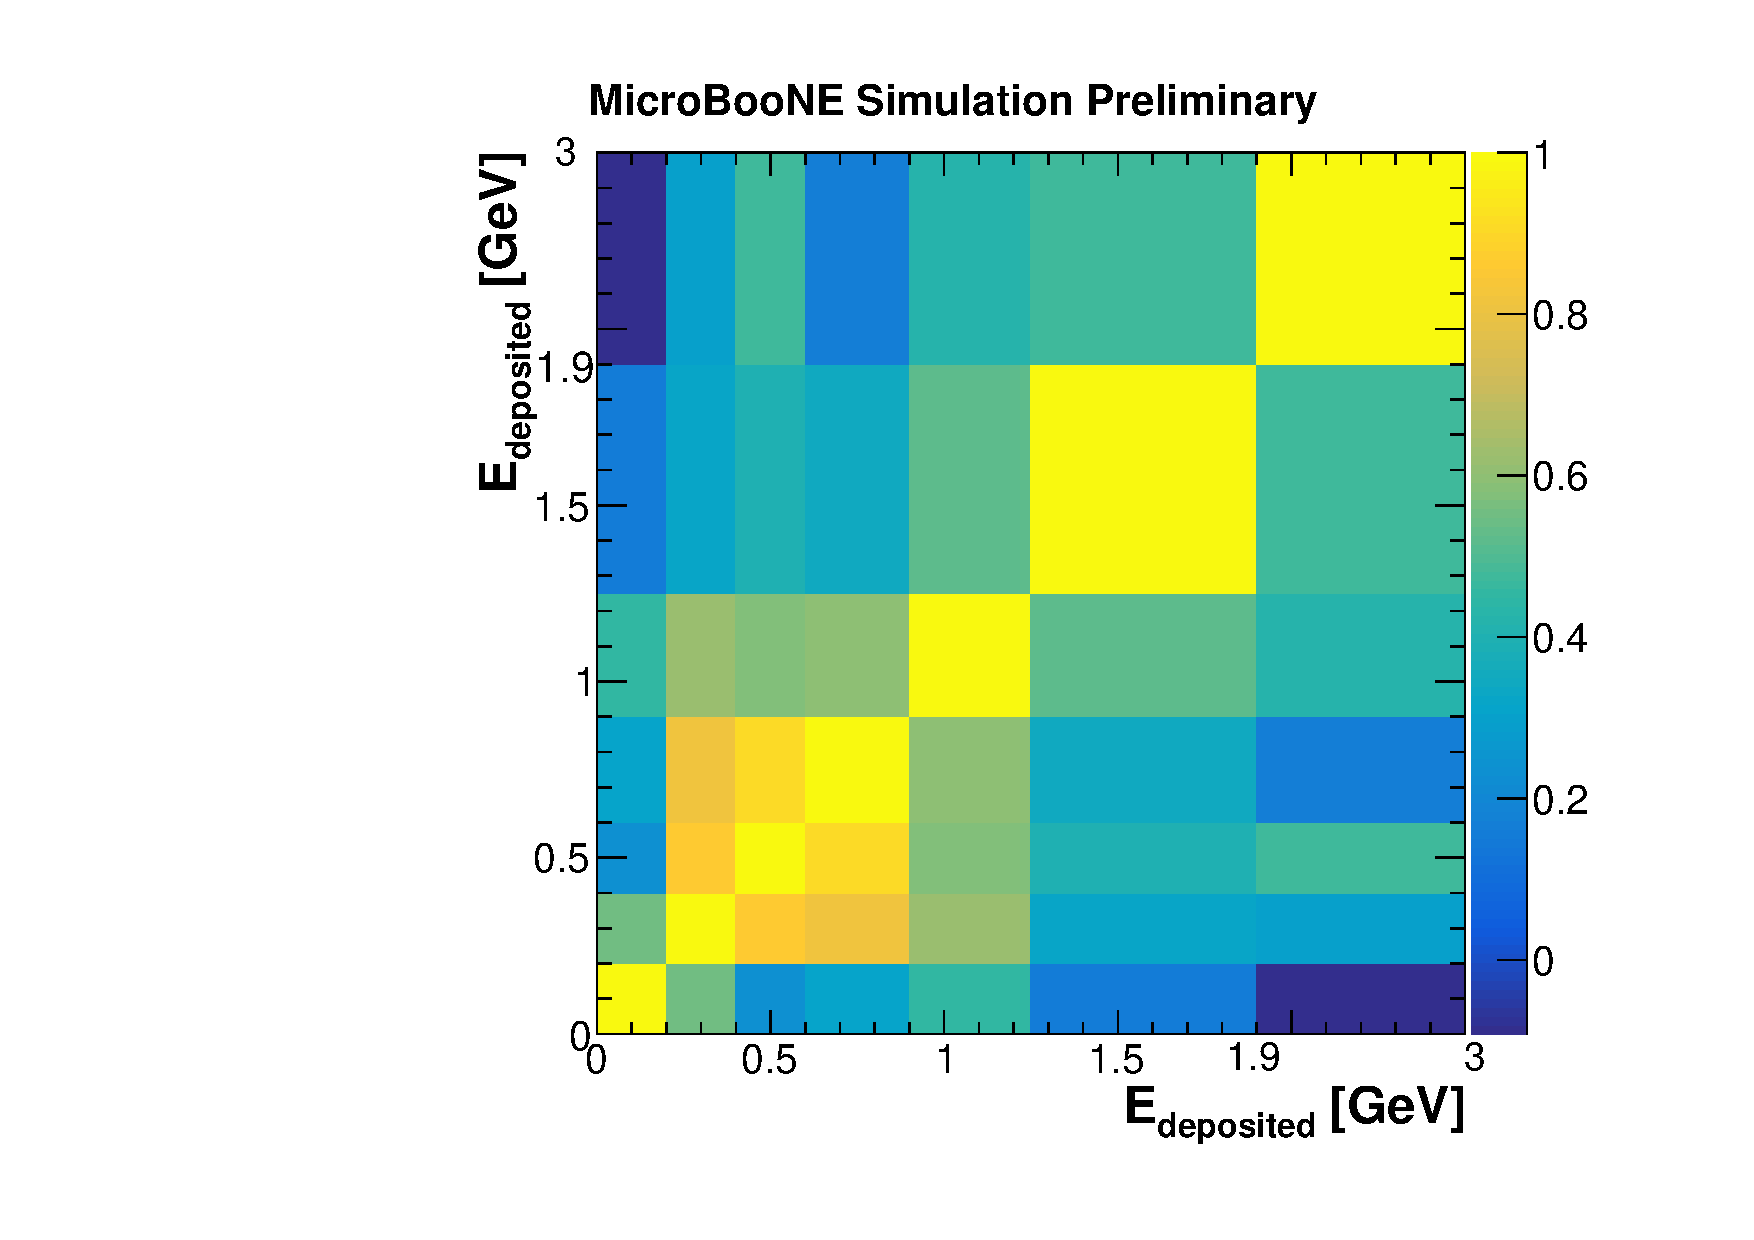
\includegraphics[width=\linewidth]{figures/corr_det.pdf}
      \caption{Correlation matrix.}  \label{fig:corr_det}
    \end{subfigure}
    \caption{Reconstructed energy spectrum, fractional covariance matrix, and correlation matrix obtained with the detector variations samples. The red bars correspond to the central value and its detector systematic uncertainty only. The data beam-off sample is not included in these plots.} \label{fig:det_sys}
	\end{center}
\end{figure}


\begin{table}[htbp]
   \centering
   \caption{Summary of the detector uncertainties variations in the BNB+cosmic sample, broken down by event category.}\label{tab:det_bkg}
   \vspace{1em}
   \begin{tabular}{
   p{0.15\linewidth}
   >{\raggedleft\arraybackslash}p{0.105\linewidth}
   >{\raggedleft\arraybackslash}p{0.105\linewidth}
   >{\raggedleft\arraybackslash}p{0.105\linewidth}
   >{\raggedleft\arraybackslash}p{0.105\linewidth}
   >{\raggedleft\arraybackslash}p{0.105\linewidth}
   >{\raggedleft\arraybackslash}p{0.105\linewidth}
   }
     \toprule
     Sample & Beam intrinsic $\nu_{\mu}$ [\%]& Beam intrinsic NC [\%]& Outside fid. vol. [\%]& Cosmic contam. [\%]& Cosmic [\%]& Total [\%]\\
     \midrule
     SCE & 8.5 & 2.9 & 32.5 & 42.0 & 28.0 & 20.3\\
     Reco. model & 3.2 & 4.9 & 14.4 & 4.0 & -3.5 &2.5\\
     DIC & -19.0 & 2.8 & 15.9 & -7.3 & -11.5 & -8.8\\
     Light sim. & 3.6 & 0.4 & 7.0 & 20.1 & -4.9 & 4.5\\
     Sat. chan. & -6.9 & 3.6 & 4.2 & -0.4 & -5.5 & -1.4\\
     $e^-$ lifetime & 9.1 & 5.2 & 21.1 & 4.0 & 6.3 & 7.0\\
     Long. diff. & 3.2 & 0.2 & 12.0 & 11.9 & -4.3 & -0.4\\
     Trans. diff. & 1.5 & 2.2 & 5.0 & 3.9 & -3.1 & 1.1\\
     Mis. chan. & -4.6 & 4.0 & 4.2 & 0.5 & -2.4 & -0.8 \\
     Wire noise & 3.4 & 3.7 & 6.0 & 5.9 & -3.0 & 0.5\\
     PE noise & -0.7 & 2.4 & 14.4 & 5.1 & -8.6 & -0.2\\
     Cryo. light & 2.9 & 2.1 & 14.3 & 3.5 & -2.9 & 1.1\\
     Wire res. & 3.9 & 4.3 & 5.0 & 3.7 & -1.1 & 2.7\\
     \bottomrule
   \end{tabular}
\end{table}

\section{Summary}
Table \ref{tab:syst_bkg} shows the uncertainty in the number of selected events before the background rejection for the cross-section, flux, and detector systematic variations, broken down by event category. There are no detector variations available for the $\nu_e$+cosmic and dirt samples. As such, at this stage, the uncertainty on these samples is assumed to be the same one of the BNB+cosmic sample.

\begin{table}[htbp]
   \centering
   \caption{Summary of the systematic uncertainties variations in the BNB+cosmic sample, break down by event category.}\label{tab:syst_bkg}
   \vspace{1em}
   \begin{tabular}{
   p{0.26\linewidth}
   >{\raggedleft\arraybackslash}p{0.22\linewidth}
   >{\raggedleft\arraybackslash}p{0.18\linewidth}
   >{\raggedleft\arraybackslash}p{0.18\linewidth}
   }
     \toprule
     Category & Cross-section [\%]& Flux [\%]& Detector [\%]\\
     \midrule
     $\nu_e$ CC0$\pi$-Np & 16.8 & 13.0 & -\\
     $\nu_e$ CC & 11.1 & 10.9 & -\\
     \midrule
     Beam intrinsic $\nu_{\mu}$ & 10.4 & 12.1 & 25.6\\
     Beam intrinsic NC & 9.5 & 12.7 & 11.9\\
     Outside fid. vol. & 8.6 & 11.0 & 51.9~\\
     Cosmic & 9.3 & 9.3 & 34.0\\
     Cosmic contaminated & 8.6 & 11.0 & 49.5\\

     \midrule
     Total & 7.9 & 12.3 & 24.0\\
     \bottomrule
   \end{tabular}
\end{table}

% Given the small contribution of these samples to the number of selected events (2.5\% of the total), this approximation is considered sufficient at this stage. 
The statistical uncertainty of the data off-beam sample is 1.0\%. 
The total uncertainty on the number of selected events, obtained with Eq. \ref{eq:cov_tot}, is 27.2~\%.

The flux and cross-section systematic uncertainties do not show a large variation among the background categories of the BNB+cosmic sample. The smallest cross-section variation is 8.6\% for the \emph{Cosmic contaminated} and \emph{Outside fid. vol.} component, while the largest is 10.4\% for the \emph{Beam intrinsic $\nu_{\mu}$} category. The flux variations span from 9.3\% for the \emph{Cosmic} events to 12.7\% for the \emph{Beam intrinsic NC} component. The flux and cross-section variations for the \emph{Cosmic} and the \emph{Cosmic contaminated} categories refer to the simulated neutrino interaction in the event, as the cosmic themselves are obviously not affected by the neutrino cross section.

The flux and cross-section uncertainties have been evaluated also for the events in the $\nu_e$ + cosmic and dirt samples. The flux (cross-section) uncertainties are 13.0\% and 10.9\% (16.8\% and 11.1\%) for the $\nu_e$~CC0$\pi$-Np and the $\nu_e$ CC events, respectively. This higher uncertainties, compared with the BNB+cosmic sample, reflect the limited $\nu_e$ cross-section measurements available. 

Figure \ref{fig:sys_tot} shows the full fractional covariance and correlation matrices obtained by combining the statistical, cross-section, flux, and detector uncertainties for the $E_{\mathrm{deposited}}$ distribution before the background rejection. The covariance matrix is used to calculate the systematic uncertainties shown in Figure \ref{fig:spectrum}. 

\begin{figure}[htbp]
  \begin{center}
    \begin{subfigure}{0.49\textwidth}
      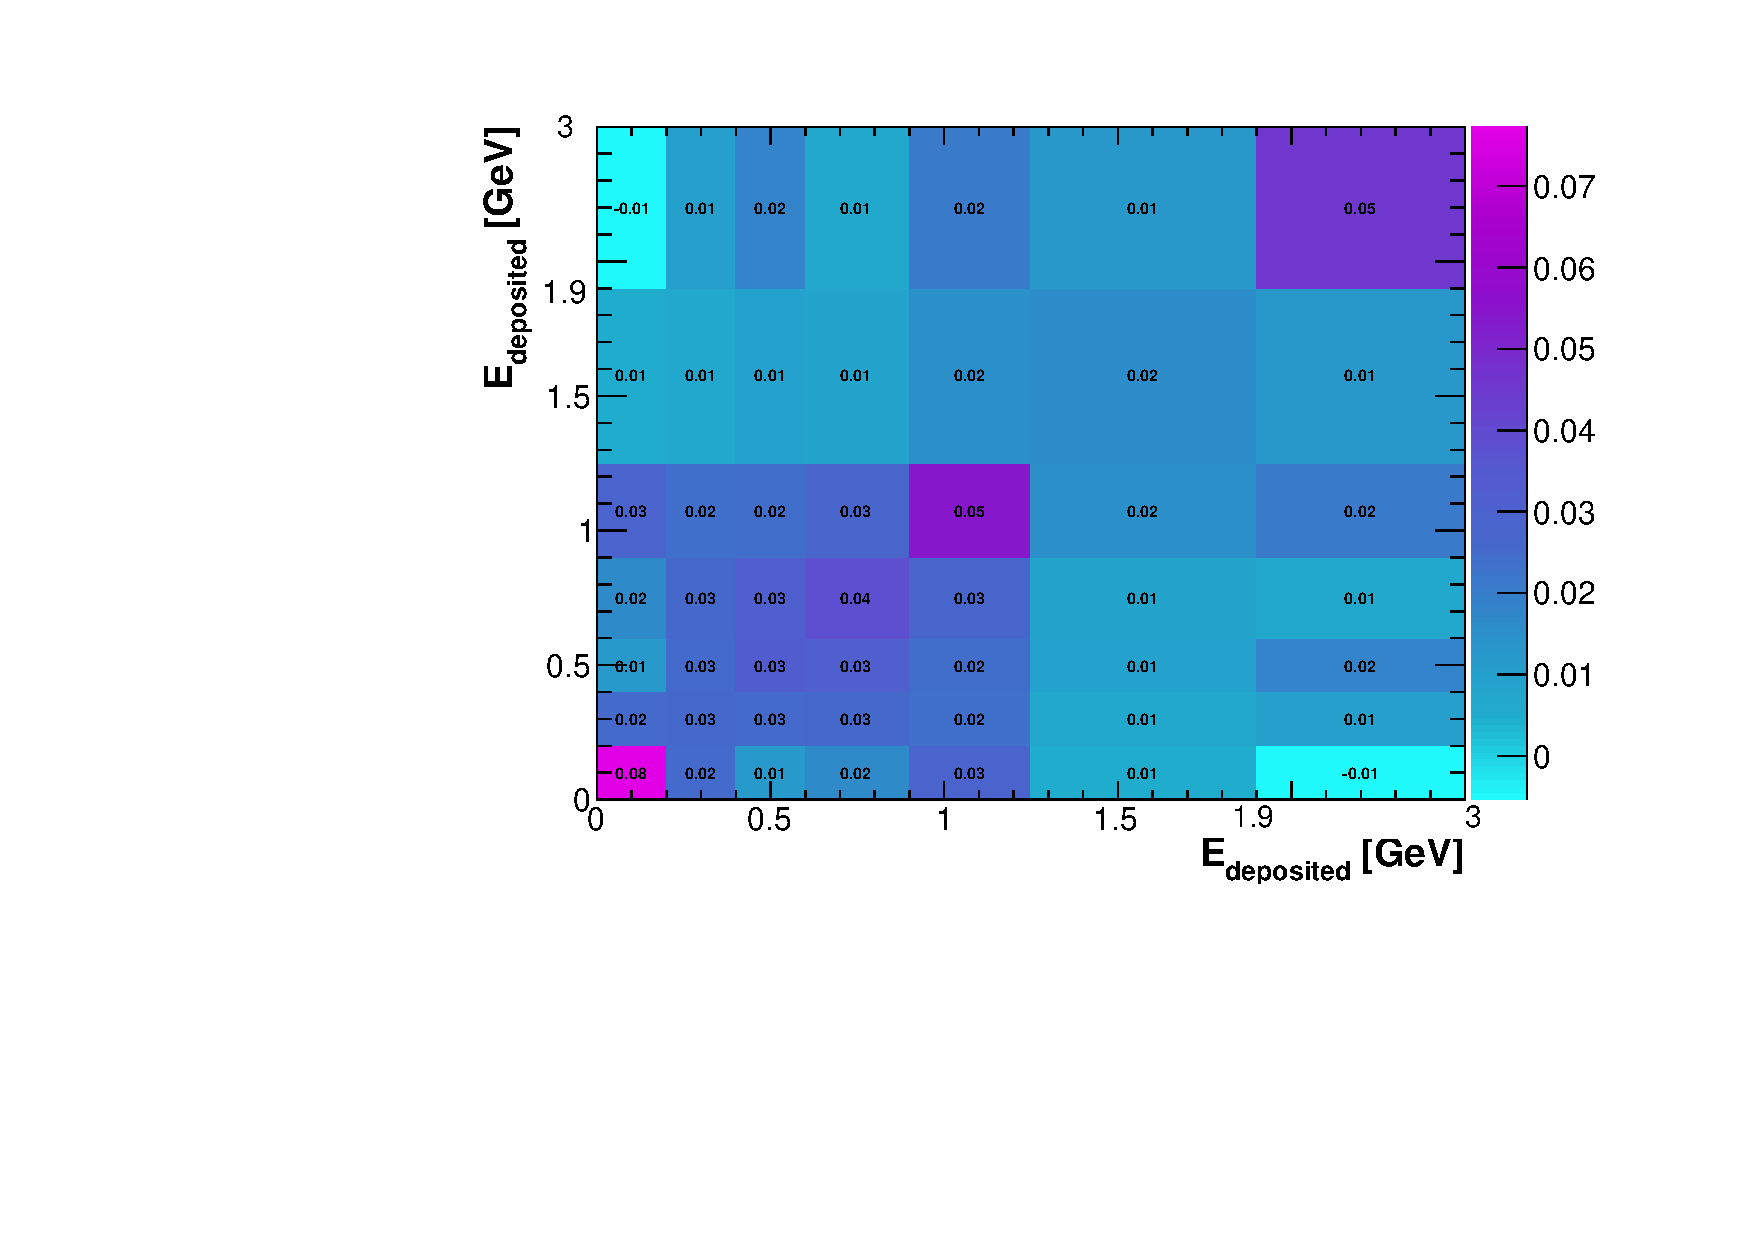
\includegraphics[width=\linewidth]{figures/h_frac_tot.pdf}
      \caption{Fractional covariance matrix.}  \label{fig:frac_tot}
    \end{subfigure}\hfill
    \begin{subfigure}{0.49\textwidth}
      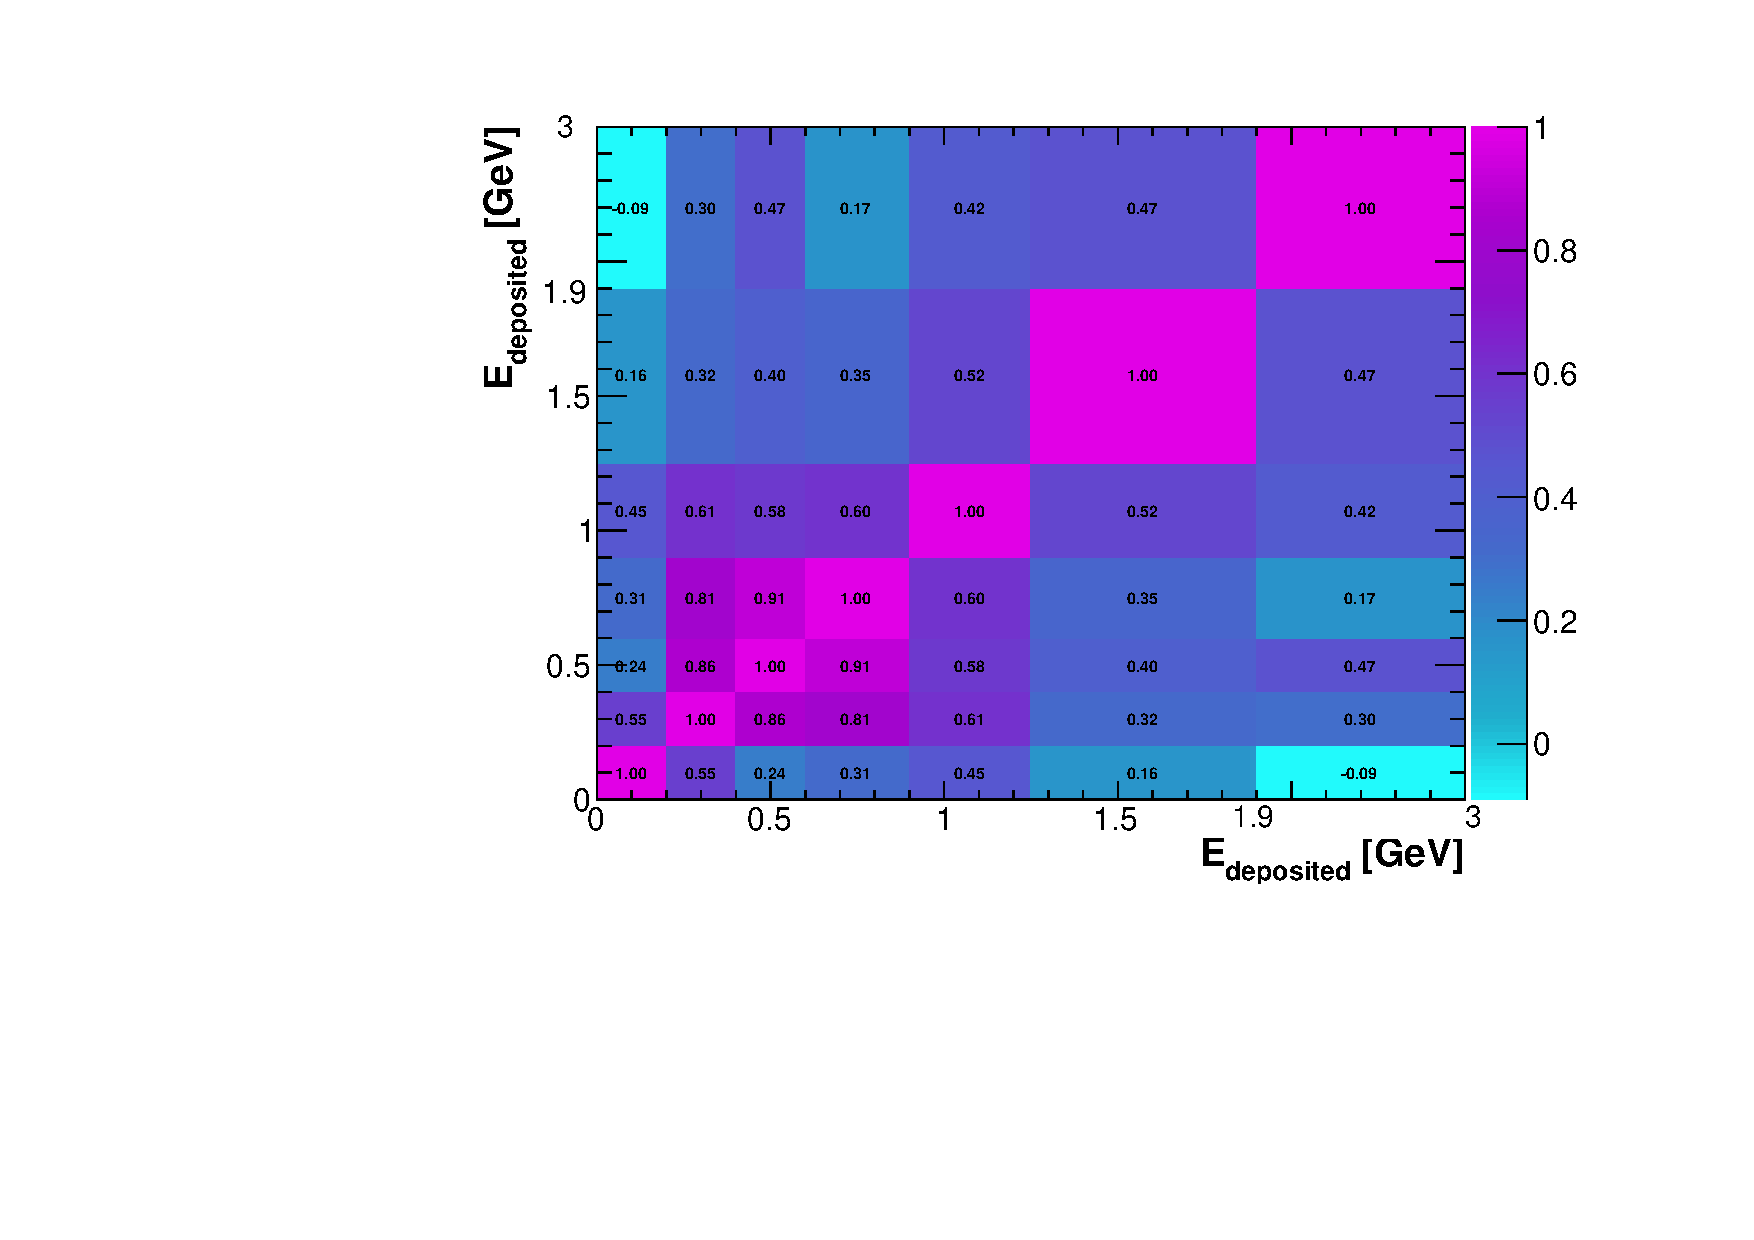
\includegraphics[width=\linewidth]{figures/h_corr_tot.pdf}
      \caption{Correlation matrix.} \label{fig:corr_tot}
    \end{subfigure}
    \caption{Full fractional covariance (left) and correlation (right) matrices obtained by combining the statistical, cross-section, flux, and detector uncertainties for the $E_{\mathrm{deposited}}$ distribution before the background rejection.} \label{fig:sys_tot}
	\end{center}
\end{figure}